
%% bare_conf_compsoc.tex
%% V1.4b
%% 2015/08/26
%% by Michael Shell
%% See:
%% http://www.michaelshell.org/
%% for current contact information.
%%
%% This is a skeleton file demonstrating the use of IEEEtran.cls
%% (requires IEEEtran.cls version 1.8b or later) with an IEEE Computer
%% Society conference paper.
%%
%% Support sites:
%% http://www.michaelshell.org/tex/ieeetran/
%% http://www.ctan.org/pkg/ieeetran
%% and
%% http://www.ieee.org/

%%*************************************************************************
%% Legal Notice:
%% This code is offered as-is without any warranty either expressed or
%% implied; without even the implied warranty of MERCHANTABILITY or
%% FITNESS FOR A PARTICULAR PURPOSE! 
%% User assumes all risk.
%% In no event shall the IEEE or any contributor to this code be liable for
%% any damages or losses, including, but not limited to, incidental,
%% consequential, or any other damages, resulting from the use or misuse
%% of any information contained here.
%%
%% All comments are the opinions of their respective authors and are not
%% necessarily endorsed by the IEEE.
%%
%% This work is distributed under the LaTeX Project Public License (LPPL)
%% ( http://www.latex-project.org/ ) version 1.3, and may be freely used,
%% distributed and modified. A copy of the LPPL, version 1.3, is included
%% in the base LaTeX documentation of all distributions of LaTeX released
%% 2003/12/01 or later.
%% Retain all contribution notices and credits.
%% ** Modified files should be clearly indicated as such, including  **
%% ** renaming them and changing author support contact information. **
%%*************************************************************************


% *** Authors should verify (and, if needed, correct) their LaTeX system  ***
% *** with the testflow diagnostic prior to trusting their LaTeX platform ***
% *** with production work. The IEEE's font choices and paper sizes can   ***
% *** trigger bugs that do not appear when using other class files.       ***                          ***
% The testflow support page is at:
% http://www.michaelshell.org/tex/testflow/



\documentclass[10pt,journal,compsoc]{IEEEtran}
% \documentclass[10pt,conference,compsoc]{IEEEtran}
% Some/most Computer Society conferences require the compsoc mode option,
% but others may want the standard conference format.
%
% If IEEEtran.cls has not been installed into the LaTeX system files,
% manually specify the path to it like:
% \documentclass[conference,compsoc]{../sty/IEEEtran}





% Some very useful LaTeX packages include:
% (uncomment the ones you want to load)


% *** MISC UTILITY PACKAGES ***
%
%\usepackage{ifpdf}
% Heiko Oberdiek's ifpdf.sty is very useful if you need conditional
% compilation based on whether the output is pdf or dvi.
% usage:
% \ifpdf
%   % pdf code
% \else
%   % dvi code
% \fi
% The latest version of ifpdf.sty can be obtained from:
% http://www.ctan.org/pkg/ifpdf
% Also, note that IEEEtran.cls V1.7 and later provides a builtin
% \ifCLASSINFOpdf conditional that works the same way.
% When switching from latex to pdflatex and vice-versa, the compiler may
% have to be run twice to clear warning/error messages.






% *** CITATION PACKAGES ***
%
\ifCLASSOPTIONcompsoc
  % IEEE Computer Society needs nocompress option
  % requires cite.sty v4.0 or later (November 2003)
  \usepackage[nocompress]{cite}
\else
  % normal IEEE
  \usepackage{cite}
\fi
% cite.sty was written by Donald Arseneau
% V1.6 and later of IEEEtran pre-defines the format of the cite.sty package
% \cite{} output to follow that of the IEEE. Loading the cite package will
% result in citation numbers being automatically sorted and properly
% "compressed/ranged". e.g., [1], [9], [2], [7], [5], [6] without using
% cite.sty will become [1], [2], [5]--[7], [9] using cite.sty. cite.sty's
% \cite will automatically add leading space, if needed. Use cite.sty's
% noadjust option (cite.sty V3.8 and later) if you want to turn this off
% such as if a citation ever needs to be enclosed in parenthesis.
% cite.sty is already installed on most LaTeX systems. Be sure and use
% version 5.0 (2009-03-20) and later if using hyperref.sty.
% The latest version can be obtained at:
% http://www.ctan.org/pkg/cite
% The documentation is contained in the cite.sty file itself.
%
% Note that some packages require special options to format as the Computer
% Society requires. In particular, Computer Society  papers do not use
% compressed citation ranges as is done in typical IEEE papers
% (e.g., [1]-[4]). Instead, they list every citation separately in order
% (e.g., [1], [2], [3], [4]). To get the latter we need to load the cite
% package with the nocompress option which is supported by cite.sty v4.0
% and later.





% *** GRAPHICS RELATED PACKAGES ***
%
\ifCLASSINFOpdf
  % \usepackage[pdftex]{graphicx}
  % declare the path(s) where your graphic files are
  % \graphicspath{{../pdf/}{../jpeg/}}
  % and their extensions so you won't have to specify these with
  % every instance of \includegraphics
  % \DeclareGraphicsExtensions{.pdf,.jpeg,.png}
\else
  % or other class option (dvipsone, dvipdf, if not using dvips). graphicx
  % will default to the driver specified in the system graphics.cfg if no
  % driver is specified.
  % \usepackage[dvips]{graphicx}
  % declare the path(s) where your graphic files are
  % \graphicspath{{../eps/}}
  % and their extensions so you won't have to specify these with
  % every instance of \includegraphics
  % \DeclareGraphicsExtensions{.eps}
\fi
% graphicx was written by David Carlisle and Sebastian Rahtz. It is
% required if you want graphics, photos, etc. graphicx.sty is already
% installed on most LaTeX systems. The latest version and documentation
% can be obtained at: 
% http://www.ctan.org/pkg/graphicx
% Another good source of documentation is "Using Imported Graphics in
% LaTeX2e" by Keith Reckdahl which can be found at:
% http://www.ctan.org/pkg/epslatex
%
% latex, and pdflatex in dvi mode, support graphics in encapsulated
% postscript (.eps) format. pdflatex in pdf mode supports graphics
% in .pdf, .jpeg, .png and .mps (metapost) formats. Users should ensure
% that all non-photo figures use a vector format (.eps, .pdf, .mps) and
% not a bitmapped formats (.jpeg, .png). The IEEE frowns on bitmapped formats
% which can result in "jaggedy"/blurry rendering of lines and letters as
% well as large increases in file sizes.
%
% You can find documentation about the pdfTeX application at:
% http://www.tug.org/applications/pdftex





% *** MATH PACKAGES ***
%
%\usepackage{amsmath}
% A popular package from the American Mathematical Society that provides
% many useful and powerful commands for dealing with mathematics.
%
% Note that the amsmath package sets \interdisplaylinepenalty to 10000
% thus preventing page breaks from occurring within multiline equations. Use:
%\interdisplaylinepenalty=2500
% after loading amsmath to restore such page breaks as IEEEtran.cls normally
% does. amsmath.sty is already installed on most LaTeX systems. The latest
% version and documentation can be obtained at:
% http://www.ctan.org/pkg/amsmath





% *** SPECIALIZED LIST PACKAGES ***
%
%\usepackage{algorithmic}
% algorithmic.sty was written by Peter Williams and Rogerio Brito.
% This package provides an algorithmic environment fo describing algorithms.
% You can use the algorithmic environment in-text or within a figure
% environment to provide for a floating algorithm. Do NOT use the algorithm
% floating environment provided by algorithm.sty (by the same authors) or
% algorithm2e.sty (by Christophe Fiorio) as the IEEE does not use dedicated
% algorithm float types and packages that provide these will not provide
% correct IEEE style captions. The latest version and documentation of
% algorithmic.sty can be obtained at:
% http://www.ctan.org/pkg/algorithms
% Also of interest may be the (relatively newer and more customizable)
% algorithmicx.sty package by Szasz Janos:
% http://www.ctan.org/pkg/algorithmicx

\usepackage{listings}
\lstset{
	language=C,
	morekeywords={iterate, until, for, every},
	basicstyle=\small\rmfamily,
	keywordstyle=\bfseries,
	numbers=left,
	columns=fullflexible,
	showstringspaces=false,
	xleftmargin=1.8em,
	frame=lines,
}




% *** ALIGNMENT PACKAGES ***
%
\usepackage{array}
% Frank Mittelbach's and David Carlisle's array.sty patches and improves
% the standard LaTeX2e array and tabular environments to provide better
% appearance and additional user controls. As the default LaTeX2e table
% generation code is lacking to the point of almost being broken with
% respect to the quality of the end results, all users are strongly
% advised to use an enhanced (at the very least that provided by array.sty)
% set of table tools. array.sty is already installed on most systems. The
% latest version and documentation can be obtained at:
% http://www.ctan.org/pkg/array


% IEEEtran contains the IEEEeqnarray family of commands that can be used to
% generate multiline equations as well as matrices, tables, etc., of high
% quality.




% *** SUBFIGURE PACKAGES ***
%\ifCLASSOPTIONcompsoc
%  \usepackage[caption=false,font=footnotesize,labelfont=sf,textfont=sf]{subfig}
%\else
%  \usepackage[caption=false,font=footnotesize]{subfig}
%\fi
% subfig.sty, written by Steven Douglas Cochran, is the modern replacement
% for subfigure.sty, the latter of which is no longer maintained and is
% incompatible with some LaTeX packages including fixltx2e. However,
% subfig.sty requires and automatically loads Axel Sommerfeldt's caption.sty
% which will override IEEEtran.cls' handling of captions and this will result
% in non-IEEE style figure/table captions. To prevent this problem, be sure
% and invoke subfig.sty's "caption=false" package option (available since
% subfig.sty version 1.3, 2005/06/28) as this is will preserve IEEEtran.cls
% handling of captions.
% Note that the Computer Society format requires a sans serif font rather
% than the serif font used in traditional IEEE formatting and thus the need
% to invoke different subfig.sty package options depending on whether
% compsoc mode has been enabled.
%
% The latest version and documentation of subfig.sty can be obtained at:
% http://www.ctan.org/pkg/subfig




% *** FLOAT PACKAGES ***
%
\usepackage{fixltx2e}
% fixltx2e, the successor to the earlier fix2col.sty, was written by
% Frank Mittelbach and David Carlisle. This package corrects a few problems
% in the LaTeX2e kernel, the most notable of which is that in current
% LaTeX2e releases, the ordering of single and double column floats is not
% guaranteed to be preserved. Thus, an unpatched LaTeX2e can allow a
% single column figure to be placed prior to an earlier double column
% figure.
% Be aware that LaTeX2e kernels dated 2015 and later have fixltx2e.sty's
% corrections already built into the system in which case a warning will
% be issued if an attempt is made to load fixltx2e.sty as it is no longer
% needed.
% The latest version and documentation can be found at:
% http://www.ctan.org/pkg/fixltx2e


\usepackage{stfloats}
% stfloats.sty was written by Sigitas Tolusis. This package gives LaTeX2e
% the ability to do double column floats at the bottom of the page as well
% as the top. (e.g., "\begin{figure*}[!b]" is not normally possible in
% LaTeX2e). It also provides a command:
%\fnbelowfloat
% to enable the placement of footnotes below bottom floats (the standard
% LaTeX2e kernel puts them above bottom floats). This is an invasive package
% which rewrites many portions of the LaTeX2e float routines. It may not work
% with other packages that modify the LaTeX2e float routines. The latest
% version and documentation can be obtained at:
% http://www.ctan.org/pkg/stfloats
% Do not use the stfloats baselinefloat ability as the IEEE does not allow
% \baselineskip to stretch. Authors submitting work to the IEEE should note
% that the IEEE rarely uses double column equations and that authors should try
% to avoid such use. Do not be tempted to use the cuted.sty or midfloat.sty
% packages (also by Sigitas Tolusis) as the IEEE does not format its papers in
% such ways.
% Do not attempt to use stfloats with fixltx2e as they are incompatible.
% Instead, use Morten Hogholm'a dblfloatfix which combines the features
% of both fixltx2e and stfloats:
%
% \usepackage{dblfloatfix}
% The latest version can be found at:
% http://www.ctan.org/pkg/dblfloatfix




% *** PDF, URL AND HYPERLINK PACKAGES ***
%
\usepackage{url}
% url.sty was written by Donald Arseneau. It provides better support for
% handling and breaking URLs. url.sty is already installed on most LaTeX
% systems. The latest version and documentation can be obtained at:
% http://www.ctan.org/pkg/url
% Basically, \url{my_url_here}.

\makeatletter
\g@addto@macro{\UrlBreaks}{\UrlOrds}
\makeatother




% *** Do not adjust lengths that control margins, column widths, etc. ***
% *** Do not use packages that alter fonts (such as pslatex).         ***
% There should be no need to do such things with IEEEtran.cls V1.6 and later.
% (Unless specifically asked to do so by the journal or conference you plan
% to submit to, of course. )


% correct bad hyphenation here
\hyphenation{
	CLCuda-API
	op-ti-cal
	net-works
	semi-conduc-tor
	re-para-meteri-zation
	bi-bli-o-gra-phy
	col-la-bo-ra-tion
	net-work
	co-pur-cha-sing
	lar-gest
}

% from SuperComputing Glasswing paper
\usepackage{epsfig}
\usepackage{amssymb}
\usepackage{amsmath}
\usepackage{amsfonts}
\usepackage{pslatex}
% \usepackage{comment}
\usepackage{verbatim}
\usepackage{dcolumn}
\newcolumntype{d}[1]{D{.}{.}{#1}}
% \usepackage[noadjust]{cite}
\usepackage{fancyhdr}
\setcounter{secnumdepth}{4}

% from distr-paper
\usepackage{epstopdf}
\usepackage{xspace}
\usepackage{defs}
\usepackage{amsthm}
\usepackage{amssymb}
\usepackage{algorithm}
\usepackage{algorithmic}
% \usepackage{comment}
% \newcolumntype{d}[1]{D{.}{.}{#1}}
\newcolumntype{C}[1]{>{\centering\arraybackslash}m{#1}}
\newcolumntype{L}[1]{>{\raggedright\arraybackslash}m{#1}}

\newcommand\Note[1]{\textbf{Note: #1}}


\begin{document}
%
% paper title
% Titles are generally capitalized except for words such as a, an, and, as,
% at, but, by, for, in, nor, of, on, or, the, to and up, which are usually
% not capitalized unless they are the first or last word of the title.
% Linebreaks \\ can be used within to get better formatting as desired.
% Do not put math or special symbols in the title.
%
% paper title
% can use linebreaks \\ within to get better formatting as desired
\title{Detecting Overlapping Communities within Graphs using an Accelerated Markov
Chain Monte Carlo Algorithm}
\title{Performance Tuning a Stochastic Gradient Markov Chain Monte Carlo
Overlapping Community Detection Algorithm}

\title{Optimizing a Markov Chain Monte Carlo Algorithm to Detect Overlapping
Communities}

\title{Accelerating Overlapping Community Detection: Performance Tuning
 a Stochastic Gradient Markov Chain Monte Carlo Algorithm}

\title{Accelerating and Scaling \\ Overlapping Community Detection}

% author names and affiliations
% use a multiple column layout for up to two different
% affiliations

\author{\IEEEauthorblockN{Ismail El-Helw\IEEEauthorrefmark{1},
Rutger Hofman\IEEEauthorrefmark{1},
Wenzhe Li\IEEEauthorrefmark{2},
Sungjin Ahn\IEEEauthorrefmark{3},
Max Welling\IEEEauthorrefmark{4} and
Henri Bal\IEEEauthorrefmark{1}\\}
\IEEEauthorblockA{\IEEEauthorrefmark{1}Vrije Universiteit Amsterdam, The Netherlands. Email: ielhelw@gmail.com, \{rutger,bal\}@cs.vu.nl \\}
\IEEEauthorblockA{\IEEEauthorrefmark{2}University of Southern California, USA. Email: wenzheli@usc.edu \\}
\IEEEauthorblockA{\IEEEauthorrefmark{3}University of Montreal, Canada. Email: sungjia@ics.uci.edu \\}
\IEEEauthorblockA{\IEEEauthorrefmark{4}University of Amsterdam, The Netherlands. Email: m.welling@uva.nl}}


% conference papers do not typically use \thanks and this command
% is locked out in conference mode. If really needed, such as for
% the acknowledgment of grants, issue a \IEEEoverridecommandlockouts
% after \documentclass

% for over three affiliations, or if they all won't fit within the width
% of the page (and note that there is less available width in this regard for
% compsoc conferences compared to traditional conferences), use this
% alternative format:
% 
%\author{\IEEEauthorblockN{Michael Shell\IEEEauthorrefmark{1},
%Homer Simpson\IEEEauthorrefmark{2},
%James Kirk\IEEEauthorrefmark{3}, 
%Montgomery Scott\IEEEauthorrefmark{3} and
%Eldon Tyrell\IEEEauthorrefmark{4}}
%\IEEEauthorblockA{\IEEEauthorrefmark{1}School of Electrical and Computer Engineering\\
%Georgia Institute of Technology,
%Atlanta, Georgia 30332--0250\\ Email: see http://www.michaelshell.org/contact.html}
%\IEEEauthorblockA{\IEEEauthorrefmark{2}Twentieth Century Fox, Springfield, USA\\
%Email: homer@thesimpsons.com}
%\IEEEauthorblockA{\IEEEauthorrefmark{3}Starfleet Academy, San Francisco, California 96678-2391\\
%Telephone: (800) 555--1212, Fax: (888) 555--1212}
%\IEEEauthorblockA{\IEEEauthorrefmark{4}Tyrell Inc., 123 Replicant Street, Los Angeles, California 90210--4321}}




% use for special paper notices
%\IEEEspecialpapernotice{(Invited Paper)}




% make the title area
\maketitle

% As a general rule, do not put math, special symbols or citations
% in the abstract
\begin{abstract}
Recent advances in machine learning algorithms have transformed the data
analytics domain and provided innovative solutions to inherently difficult
problems. However, achieving good performance while training models at scale over large
data sets remains a
daunting challenge. One such problem is the detection of overlapping
communities within graphs. For example, a social network can be modeled as a
graph where the vertices and edges represent individuals and their
relationships. In contrast to the problem of graph partitioning or clustering, an
individual can be part of multiple communities which significantly increases
the problem complexity.
% same as above:
% Accelerating sequential algorithms in order to achieve high performance is
% often a nontrivial task. However, there are certain properties that can
% exacerbate this process and make it particularly daunting. For example,
% building an efficient parallel solution for a data-intensive algorithm requires
% a deep analysis of the memory access patterns and data reuse potential. In this
% context, the optimization landscape can be extremely complex owing to the large
% number of trade-off decisions.

In this paper, we discuss our experience in accelerating and scaling an existing
data-intensive algorithm for overlapping community detection.
As our first contribution, we present our methodology and findings in parallelizing the
computation using multiple classes of GPUs.
Analysis of the algorithm's computation and data dependencies resulted in a
75\% reduction in its memory footprint and data intensity. We
employed a customizable code generation strategy to thoroughly explore the
optimization design space and identify the
optimal combination of optimizations for each compute device. We present an
empirical evaluation and show that the parallelization
achieves speedups of up to 120$\times$ compared to an already optimized sequential
version.

As our second contribution, we scale this algorithm out towards very large data sets, where memory
requirements become the foremost bottleneck. Our solution is an efficient
parallel and distributed implementation. We show that the algorithm can
scale and process graphs consisting of billions of edges and tens of millions
of vertices on a compute cluster of 65 nodes. To the best of our knowledge,
this is the first time that the problem of deducing overlapping communities
has been learned for problems of such a large scale.

\end{abstract}

% no keywords
\begin{IEEEkeywords}
    Algorithms for Accelerators and Heterogeneous Systems;
%
    Distributed Computing;
    % Parallel Programming;
    High-performance computing;
%
    Performance Analysis;
%
    Combinatorial and Data Intensive Application;
    Statistical Learning.
\end{IEEEkeywords}




% For peer review papers, you can put extra information on the cover
% page as needed:
% \ifCLASSOPTIONpeerreview
% \begin{center} \bfseries EDICS Category: 3-BBND \end{center}
% \fi
%
% For peerreview papers, this IEEEtran command inserts a page break and
% creates the second title. It will be ignored for other modes.
\IEEEpeerreviewmaketitle


\section{Introduction}
The tremendous amount of data that we generate through our daily applications such as social networking services, online shopping, and news recommendations, provides us with an opportunity to extract hidden but useful, even invaluable information. Realizing this opportunity, however, requires a significant amount of effort because traditional machine learning algorithms often become extremely inefficient with large amounts of data.

There have been two main approaches to resolving this issue; machine learning researchers have developed new scalable algorithms~\cite{bottou2010large, boyd2011distributed}, while systems and networking researchers have worked on developing new generic infrastructure systems which can be leveraged to construct machine learning solutions more efficiently~\cite{dean2008mapreduce, chang2008bigtable}.
However, the best possible performance is often achieved by carefully integrating both of these approaches in a single solution.

One such big data problem is analyzing large graphs such as social networks where it is not unusual to see a network consisting of billions of edges and tens of million of vertices~\cite{yang2015defining}. In particular, we are interested in the overlapping community detection problem~\cite{xie2013overlapping}, where the goal is to learn the probability distribution of each vertex to participate in each community, given a set of vertices, the links between them (which are usually very sparse), and the number of latent communities. A community can be seen as a densely connected group of vertices that are only sparsely connected to the rest of the network. This problem is significantly more complex than the related domain of detecting disjoint communities.

The problem of detecting overlapping communities is modeled by the mixed membership stochastic block model (MMSB)~\cite{airoldi2009mixed} and in this paper we are particularly interested in a variant of MMSB, called assortative MMSB (a-MMSB\footnote{Although we work on a-MMSB for simplicity, it is also straightforward to apply the proposed method to the general MMSB model.}) \cite{gopalan2012scalable}.
The MMSB model is a probabilistic graphical model~\cite{koller2009probabilistic} that represents a convenient paradigm for modeling complex relationships between a potentially large number of random variables. Bayesian graphical models, where we define priors and infer posteriors over parameters, also allow us to quantify model uncertainty and facilitate model selection and averaging. However, an increasingly urgent question is whether these models and their inference procedures will be up to the challenge of handling very large graphs.

There have been two main recent advances in this direction of scalable Bayesian inference: methods based on stochastic variational Bayes (SVB)~\cite{gopalan2012scalable,hoffman2013stochastic,gopalan2013efficient} and stochastic gradient Markov chain Monte Carlo (SG-MCMC)~\cite{welling2011bayesian,patterson2013stochastic,ahn2014distributed,ahn2012bayesian}. Both methods have the important property that they only require a small subset of the data for every iteration. In other words, they can be applied to (infinite) streaming data.

In this paper, we focus on the SG-MCMC method applied to the a-MMSB model. Recent
work of the authors of this paper~\cite{LiAW15} showed that this methodology is faster and more accurate than the
SVB method. That work further proposes a heuristic to scale up the number of
communities at the cost of less precision; the work in this paper considers the
algorithm without that heuristic.

From a computational point of view, our SG-MCMC a-MMSB algorithm differs
from widespread machine learning algorithms like deep learning in several
ways. First, it is \emph{highly data-intensive} which makes parallel acceleration
particularly challenging. Second, owing to the algorithm's stochastic
nature, the majority of its memory access patterns and data dependencies
are non-deterministic. As a result, straightforward optimization attempts
of the memory access patterns either fail or lead to non-intuitive results. Third,
the size of its intermediate data structures makes it difficult to scale to very large
community graphs.

Starting from an existing implementation in Python/Numpy, we create an efficient
C++ version to serve as the baseline for the parallel versions.
This already improves performance by a factor of 1000 to 1500 compared to
Python.
% This transformation is not considered one of our key contributions.
Then, our key contributions to the algorithm are:

\begin{itemize}
\item \textbf{scaling up to run on GPUs.}
The application is not a natural fit for GPUs, because it is data-bound and
irregular in its data accesses. Nevertheless, we developed aggressive
memory allocation optimizations to solve the data bandwidth issues for GPUs.
This implementation achieves up to 86$\times$ speedup compared to the baseline.
%
We managed to reduce the algorithm's memory requirements by roughly 75\%, which
significantly reduces the data intensity and allows for tackling larger
problems; % while maintaining all state in memory.

\item \textbf{scaling out to overcome the memory bounds posed by GPUs} or,
generally, single-machine systems, to solve the largest publicly available
community graphs. % This necessitated overcoming several challenges.
% The algorithm's state grows rapidly with larger graphs and number of latent
% communities.
Since the full state for the larger graphs does not fit in a
single machine's memory, it is partitioned across a cluster
of machines. Hence, the cluster nodes must read
remote memory hosted by their peers. Since the algorithm is data-bound, we
substantially optimized remote memory accesses by implementing
a custom RDMA store.
On top of that, we pipelined the algorithm stages by fetching
data in advance over the network;
\begin{comment} Finally, the algorithm's computation
is effectively distributed across the cluster nodes and parallelized further
within each node by exploiting their multi-core CPUs.
\end{comment}

\item \textbf{the use of pipelining} \emph{in the distributed implementation}
justifies straightforward intra-node thread parallelism, and it is pointless
to combine the GPU implementations
into it. The cause is that computing for an iteration takes less
time than fetching the data from remote memory, and the computation is
fully overlapped with fulfilling the data requests for the next iteration.
Hence, it is useless to improve the computation time.

\end{itemize}
% To this end, we propose a design of a parallel and distributed system specifically tailored to solve the a-MMSB problem. In particular, we use a mixture of OpenMP, MPI and RDMA in order to efficiently scale and accelerate the algorithm's computation.

\begin{comment}
Further, by cataloguing and accounting for the various load and store
operations, we identified the highest priority locations of data reuse. In
order to circumvent the unclear optimization landscape, we developed an
effective kernel code generation mechanism that explores the benefits of
exploiting all permutations of the available optimization opportunities. These
optimizations include caching in shared memory, caching in the register file,
loop unrolling and explicit vectorization.
\end{comment}

A bird's eye-view of the work in this paper, without any technical detail, has been
published at CCGrid-2016~\cite{10.1109/CCGrid.2016.98}.
The results of our distributed MCMC-aMMSB implementation
have been previously published at the 2016 ParLearning
workshop~\cite{DBLP:conf/ipps/El-HelwHLAWB16}, where it earned a best-paper
award.

The remainder of this paper is organized as follows.
Section~\ref{sec-background} provides an overview of the
algorithm and its theoretical foundation, with related work in
Section~\ref{sec-related}. Section~\ref{sec-design-sequential} describes how we
arrived at an efficient sequential version that serves as the baseline for the
parallel implementations. Section~\ref{sec-gpu} delves
into the parallelization optimizations for GPUs.
Section~\ref{sec-distr} describes the design, implementation and evaluation of
the scalable distributed solution. Finally, Section~\ref{sec-conclusion}
provides concluding remarks.

% -------\\
% Community detection is the central problem in network analysis, with the goal of identifying the groups of related nodes that are densely connected within this group but sparsely connected to the rest of the network. Different from classical community detection problem where we assume each node belongs to one single community, our paper considers overlapping communities where each of the nodes might belong to multiple communities. In particular, we consider the model called a-MMSB(Assortive Mixed Membership Stochastic Blockmodel) in this paper, which was first introduced in~\cite{gopalan2012scalable}.\\


% a-MMSB, as a probabilistic graphical model, represents a convenient paradigm for modeling complex relationships between a potentially large number of random variables. It also uses priors and posteriors to quantify model uncertainty and facilitate model selection and averaging. While a-MMSB provides rich representation power, like other Bayesian models, the inference procedures of handling big data which is common in real world is still a very challenging problem. \\



% Consider the large networks such as a social network, it easily runs into billions of edges and tens of million of nodes. In addition to that, the number of communities might exceed few millions. 
% There were two types of scalable algorithm for a-MMSB have been introduced recently \cite{gopalan2012scalable}, stochastic variational Bayesian inference (SVB) and stochastic gradient Markov chain Monte Carlo(SG-MCMC), respectively. Both methods have the important property that each iteration only relies on a small subset of the data. Although both methods can work for some large networks with many hundreds of nodes, the performance is far less satisfactory when it applies to the so-called "big data" such as facebook network with millions of nodes and billions of edges. Given the facts that \cite{LiAW15}, SG-MCMC runs faster and converges to the better local minima, in this paper, we mainly consider the problem of scaling up SG-MCMC to the big data set.  \textit{As far as we know, this is the first paper that studies community detection on the frencter dataset with few billion's of edges.}







\newcommand{\Vertices}{\ensuremath{\cV{}}\xspace}
\newcommand{\Edges}{\ensuremath{\cE{}}\xspace}
\newcommand{\Heldout}{\ensuremath{\cE_h{}}\xspace}
\newcommand{\SGLDMinibatch}{\ensuremath{\cD_n{}}\xspace}
\newcommand{\Minibatch}{\ensuremath{\cE_n{}}\xspace}
\newcommand{\Minibatcht}{\ensuremath{\cE_n{}}\xspace}
\newcommand{\Neighbors}{\ensuremath{\cV_n{}}\xspace}

\section{Background and Related Work}
\label{sec-background}
% In this section, we briefly review the Bayesian model we are considering in this paper.

% In this section, we briefly review the Bayesian model we are considering in this paper.
\subsection{Assortative Mixed-membership Stochastic Blockmodels (a-MMSB)}
The assortative mixed membership stochastic blockmodel (a-MMSB)~\cite{gopalan2012scalable} is a special case of MMSB~\cite{airoldi2009mixed} that models the group structure in a network of $N$ vertices. Consider a set  \Vertices containing all the vertices in the graph, and a set \Edges containing all the linked edges between pairs of vertices. Each vertex $a$ in the vertex set \Vertices has a $K$-dimensional probability distribution $\pi_a$ of participating in the $K$ members of the community set $\cK$.  For every possible peer $b$ in the network, each vertex $a$ randomly draws a community $z_{ab}$. If a pair of vertices ($a,b$) in the edge set \Edges are in the same community, i.e., $z_{ab}=z_{ba} = k$, then they have a significant probability $\bt_k$ to connect, i.e., $y_{ab}=1$. Otherwise this probability is a small value $\dt$. Each community has its connection strength $\beta_{k} \in (0,1)$ which reflects how likely its members are linked to each other. The whole generative process of a-MMSB is then described by:
\benum
\item For each community $k$, draw community strength $\bt_k \sim \mbox{Beta}(\eta)$
\item For each vertex $a$, draw community memberships $\pi_a \sim \mbox{Dirichlet}(\al)$
\item For each pair of vertices $a$ and $b$,
\benum
	\item Draw interaction indicator $z_{ab} \sim \pi_a$
    \item Draw interaction indicator $z_{ba} \sim \pi_b$
    \item Draw link $y_{ab} \sim \mbox{Bernoulli}(r)$, where $r = \bt_k$ if $z_{ab}=z_{ba}=k$, and $r=\dt$ otherwise.
\eenum
\eenum
$\eta$ and $\alpha$ are parameters to the Beta and Dirichlet distribution functions.

\subsection{Stochastic Gradient Markov Chain Monte Carlo}
The algorithm we are working on in this paper is based on stochastic gradient Langevin dynamics (SGLD)~\cite{welling2011bayesian}. SGLD applies the following update rule to obtain samples from a posterior distribution $p(\ta|\cX) \propto p(\cX|\ta) p(\ta)$ of $N$ i.i.d. data points $\cX=\{x_i\}_{i=1}^{N}$:
\bea
\ta^* \law \ta + \f{\epsilon_t}{2}\left(\nabla_{\ta}\log p(\ta_t)+N\bar{g}(\ta;\SGLDMinibatch)\right) + \xi_t, \label{eqn:sgld_update}
\eea
where $\xi_t \sim \cN(0,\epsilon_t )$ with $\ep_t$ the step size, $\SGLDMinibatch$ a mini-batch of size $n$ sampled from $\cX$, and $\bar{g}(\ta;\SGLDMinibatch)$ the mean stochastic gradient, i.e., $\frac{1}{|\SGLDMinibatch|}\sum_{x\in \SGLDMinibatch}^{}\grad_{\ta} \log p(x|\ta)$. As the step size goes to zero by a schedule satisfying $\sm{t}{\infty}\ep_t = \infty$ and $\sm{t}{\infty}\ep_t^2 < \infty$, SGLD samples from the true posterior distribution. One benefit of using SGLD is that we do not need the Metropolis-Hastings (MH) accept-reject tests since the rejection probability goes to zero as the step size tends to zero. Although in practice we often do not reduce the step size to zero to obtain better mixing (thus resulting in some bias), we obtain good performance by drawing many more samples per unit time. 

SGLD originated from Langevin Monte Carlo (LMC)~\cite{girolami2011riemann}, where unlike SGLD the gradient is computed exactly by using all data points. Then, Metropolis-Hastings accept-reject tests are applied. Comparing to LMC, SGLD only requires to process a mini-batch $\SGLDMinibatch$ at each iteration and ignores the MH test, and thus computation complexity substantially reduces from $\cO(N)$ to $\cO(n)$.   

\looseness=-1
Stochastic gradient Riemannian Langevin dynamics (SGRLD)~\cite{patterson2013stochastic} is a subclass of SGLD which is developed to efficiently sample from the probability simplex. By applying Riemannian geometry~\cite{girolami2011riemann} and using the mini-batch-based estimator in Eq.~\ref{eqn:sgld_update}, it achieved state-of-the-art performance for latent Dirichlet allocation (LDA)~\cite{blei2003latent}. In particular, for a $K$-dimensional probability simplex $\pi$, it uses the \textit{expanded-mean} re-parameterization trick, where the probability of a category $k$ is given by $\pi_k = \ta_k / \sum_{j=1}^K \ta_j$ with $\ta_k \sim \text{Gamma}(\al,1)$ and $\al$ a hyperparameter of the Dirichlet distribution $p(\pi | \al )$. Then, the update rule of SGRLD is:
\bea
\ta_{k}^* \law \left| \ta_{k} + \f{\ep_t}{2} \left( \al - \ta_{k} + \f{N}{|\SGLDMinibatch|} \sum_{d \in \SGLDMinibatch} g_d(\ta_{k}) \right) + (\ta_{k})^\ha \xi_{t} \right|, \label{eqn:sgrld_update}
\eea
here $g_d(\ta_{k})$ is the gradient of the log posterior w.r.t. $\ta_{k}$ on a data point $d\in \SGLDMinibatch$.

\addtolength{\tabcolsep}{-3pt}
\renewcommand{\arraystretch}{1.5}
\begin{table}[tb] % [htbp]
\center
\begin{tabular}{c C{0.075\textwidth} c L{0.26\textwidth}}
\textbf{symbol}
	 & \textbf{type} & \textbf{size} & \textbf{description} \\
         % & \multicolumn{1}{c}{\textbf{type}}
                           % & \multicolumn{1}{c}{\textbf{description}} \\
\hline
$\cK$      &              & $K$        & set of communities \\
\Vertices  & \{vertex\}   & $N$          & vertices in the graph \\
\Edges     & \{edge\}     &              & linked edges in the graph \\
$E$        & \{edge\}     &              & $\Vertices\times\Vertices$: linked and nonlinked edges \\
\Heldout   & \{edge\}     &              & held-out subset of the graph \\
\Minibatch & \{edge\}     &              & sampled mini-batch of edges in~$E$ \\
$M$        &              &              & number of vertices in \Minibatch \\
\Neighbors & \{vertex\}   &              & sampled neighbor set for a vertex in~\Minibatch \\
$\theta$   & float~vector 2-D & $K\times{}2$ & reparameterization of $\beta$.
					$\beta[k] = \theta[k][1] / \sum_j\theta[k][j]$ \\
$\beta$    & float vector & $K$          & community strength \\
$\phi$     & float~vector 2-D & $N\times{}K$ & reparameterization of $\pi$.
					$\pi[i][k] = \phi[i][k] / \sum_j\phi[i][j]$ \\
$\pi$      & float~vector 2-D & $N\times{}K$ &
					$\pi[i][k]$~is~probability that vertex $i$ is in community $k$ \\
\hline
\\[-3ex]
\end{tabular}
\caption{Definition of most important symbols}
\label{tbl-symbols}
\end{table}
\addtolength{\tabcolsep}{3pt}
\renewcommand{\arraystretch}{1.0}


\subsection{Scalable MCMC for a-MMSB}
This section describes the SG-MCMC algorithm for a-MMSB. Please refer to~\cite{LiAW15} for more details. The algorithm iterates updating local parameter $\pi$ and global parameter $\beta$. Since both parameters lie on the probability simplex, SGRLD is applied to make the sampling process more efficient. Here, the parameters $\phi$ and $\ta$ are used to re-parameterize $\pi$ and $\beta$ respectively. After updating $\phi$ and $\ta$, we can obtain $\pi$ and $\beta$ by normalizing $\phi$ and $\ta$ respectively, see Table~\ref{tbl-symbols}. In the following, we briefly sketch the iterative update steps.

\paragraph*{\textbf{Sampling global parameters}} the update rule for global parameter $\theta$ is
\bea
\ta_{ki}^* \law \left| \ta_{ki} + \f{\ep}{2} \left( \eta - \ta_{ki} + h(\Minibatcht)\sum_{(a,b) \in \Minibatcht}g_{ab}(\ta_{ki})\right) \right.\nn \\ \left.+ (\ta_{ki})^{\ha}\xi_{ki} \right|, \label{eqn:global_update}
\eea
where the gradient in $\theta$ is
\bea
g_{ab}(\ta_{ki})
&=& \f{f_{ab}^{(y)}(k,k)}{Z_{ab}^{(y)}} \left(\f{|1-i-y|}{\ta_{ki}} - \f{1}{\sum_j\ta_{kj}} \right),
\eea
here $\Minibatcht$ is a mini-batch of $n_t$ vertex pairs sampled from $\Edges$ or $E$; $h(\Minibatcht)$ is a weight factor to scale the effect of a mini-batch towards the full network; and 
\bea
f_{ab}^{(y)}(k,l)=
\begin{cases}
\bt_k^y(1-\bt_k)^{(1-y)}\pi_{ak}\pi_{bk}, & \mbox{if } k=l\\
\dt^{y}(1-\dt)^{(1-y)} \pi_{ak} \pi_{bl}, & \mbox{if } k \neq l \nn.
\end{cases}
\label{eqn:case}
\eea
$Z_{ab}^{(y)}$ is the normalization constant which we can compute in $\cO(K)$ time \cite{LiAW15}.

\paragraph*{\textbf{Sampling local parameters}}
the update rule for the local parameters $\phi$ is
\bea
\phi_{ak}^* \law \left| \phi_{ak} + \f{\ep}{2} \left( \al - \phi_{ak} + \f{N}{|\Neighbors|} \sum_{b \in \Neighbors} g_{ab}(\phi_{ak})\right) \right. \nn \\ \left. + (\phi_{ak})^{\ha} \xi_{ak}\right|,
\label{eqn:local_update}
\eea
where the gradient in $\phi$ is
\bea
g_{ab}(\phi_{ak}) = \f{f_{ab}^{(y)}(k)}{Z_{ab}^{(y)}\phi_{ak}} - \f{1}{\sum_j\phi_{aj}}.
\eea
Here, $\Neighbors$ is the neighbor set for a mini-batch node, another random mini-batch of $n$ nodes sampled from \Vertices. Note that $|\Neighbors| \ll |\Vertices|=N$.

As is common in machine learning problems, the edges of the graph are divided
into two sets, the training set and a held-out set \Heldout.
As the performance metric we use perplexity, which is defined as the exponential
of the negative average log-likelihood of the held-out set \Heldout. Given a collection of $T$
samples of the model parameters $\{\bt_t\}$ and $\{\pi_t\}$, the averaged
perplexity on the held-out set $\Heldout$ is 
\begin{align}
&\text{perp}_{\text{avg}}(\Heldout|\{\beta_t\},\{\pi_t\})\nonumber \\=&
\exp\left(-\frac{\sum_{(a,b)\in \Heldout}^{}\log
\{(1/T)\sm{t}{T}p(y_{ab}|\beta_t,\pi_t)\}}{|\cE_{h}|}\right).
\end{align}
The perplexity is not evaluated at every iteration, but at regular intervals.
Convergence is reached when the perplexity changes by less than a small
threshold.

The pseudo-code of the sequential algorithm is presented in Algorithm~\ref{algorithm}. 

\begin{algorithm}[t]
\caption{Sequential version of SG-MCMC for a-MMSB}\label{alg}
\begin{algorithmic}[1]
\STATE Initialize $\pi , \bt, \phi, \ta$
\WHILE {sampling}
\STATE Sample mini-batch of vertex pairs \Minibatch from \Edges or $E$
\FOR {each vertex in \Minibatch}
    \STATE Sample mini-batch of vertices $\Neighbors$ from $\Vertices$
    \STATE \texttt{update\_phi:} Update $\phi_{a}$ using Eq.~\ref{eqn:local_update} \ENDFOR
  %  $\phi_{a}^* \law \left| \phi_{a} + \f{\ep_{\phi}}{2} \left( \al - \phi_{a} + \f{N}{|\Neighbors|} \sum_{b \in \Neighbors} G_{\phi_{a}}\right) + (\phi_{a})^{\ha} \xi_{a}\right|$
\FOR {each vertex in \Minibatch}
    \STATE \texttt{update\_pi:} Obtain $\pi_a$ from $\phi_a^*$ \ENDFOR
\FOR {$k = 1,\dots,K$}
    \STATE \texttt{update\_theta:} Update $\ta_{k}$ using Eq.~\ref{eqn:global_update} \ENDFOR
\FOR {$k = 1,\dots,K$}
   % $\ta_{k}^* \law \left| \ta_{k} + \f{\ep_\ta}{2} \left( \eta - \ta_{k} + h(\cE_t) \sum_{(a,b) \in \cE_t} G_{\ta_{k}}(a,b) \right) + (\ta_{k})^{\ha}\xi_{k} \right|$
    \STATE \texttt{update\_beta:} Obtain $\bt_k$ from $\ta_k^*$ \ENDFOR
\ENDWHILE
\end{algorithmic}
\label{algorithm}
\end{algorithm}


\begin{comment}
Assortative mixed-membership stochastic blockmodel (a-MMSB) [1] is a special case of MMSB [8] that models the group-structure in a network of $N$ nodes. In particular, each node $a$ in the node set \Vertices has a $K$-dimension probability distribution $\pi_a$ of participating in the $K$ members of the community set $\cK$. For every possible peer $b$ in the network, each node $a$ randomly draws a community $z_{ab}$. If a pair of nodes ($a,b$) in the edge set \Edges are in the same community: $z_{ab}=z_{ba} = k$, then they have a significant probability $\bt_k$ to connect, i.e., $y_{ab}=1$. Otherwise this probability is small. Each community has its connection strength $\beta_{k} \in (0,1)$ which explains how likely its members are linked to each other.  

The generative process of a-MMSB is then given by,

\benum
\item For each community $k$, draw community strength $\bt_k \sim \mbox{Beta}(\eta)$
\item For each node $a$, draw community memberships $\pi_a \sim \mbox{Dirichlet}(\al)$
\item For each pair of nodes $a$ and $b$,
\benum
	\item Draw interaction indicator $z_{ab} \sim \pi_a$
    \item Draw interaction indicator $z_{ba} \sim \pi_b$
    \item Draw link $y_{ab} \sim \mbox{Bernoulli}(r)$, where $r = \bt_k$ if $z_{ab}=z_{ba}=k$, and $r=\dt$ otherwise.
\eenum
\eenum

Unlike the a-MMSB, the original MMSB maintains pair-wise community strength $\bt_{k,k'}$ for all pairs of the communities. Note that it is trivial to extend the results that we obtain in this paper to the general MMSB model. The joint probability of the above process can be written as:
\begin{align}
p(y,z,\pi ,\bt | \al, \eta) &= \prod_{a=1}^{N} \prod_{b > a}^{N} p(y_{ab} | z_{ab}, z_{ba}, \bt) p(z_{ab}|\pi_a)\nonumber \\ &p(z_{ba}|\pi_b) \pd{a}{N}p(\pi_a|\al) \pd{k}{K} p(\bt_k|\eta).\label{eqn:joint}
\end{align}

Both variational inference [1,4,16] and collapsed Gibbs sampling algorithms [11] have been used successfully for small to medium scale problems. However, the $\cO(N^2)$ computational complexity per update prevents it from being applied to large scale networks. A stochastic variational algorithm was developed in [1] to address this issue, where each update only depends on a small mini-batch of the nodes in the network. 


%%%%%%%%%%%%%%%%%%%%%%%%%%%%%%%%%%%%%%%%%%%%%%%%%%%%%%%%%%%%%%%
\section{Stochastic Gradient MCMC Algorithms}
Our algorithm will be based on the stochastic gradient Langevin dynamics (SGLD) [3]. To sample from a posterior distribution $p(\ta|\cX) \propto p(\cX|\ta) p(\ta)$ given $N$ i.i.d. data points $\cX=\{x_i\}_{i=1}^{N}$, SGLD applies the following update rule:
\bea
\ta^* \law \ta + \f{\epsilon_t}{2}\left(\nabla_{\ta}\log p(\ta_t)+N\bar{g}(\ta;\SGLDMinibatch)\right) + \xi, \label{eqn:sgld_update}
\eea
where $\xi \sim \cN(0,\epsilon_t )$ with $\ep_t$ the step size, $\SGLDMinibatch$ a mini-batch of size $n$ sampled from $\cX$, and $\bar{g}(\ta;\SGLDMinibatch) = \frac{1}{|\SGLDMinibatch|}\sum_{x\in \SGLDMinibatch}^{}\grad_{\ta} \log p(x|\ta)$. As the step size goes to zero by a schedule satisfying $\sm{t}{\infty}\ep_t = \infty$ and $\sm{t}{\infty}\ep_t^2 < \infty$, SGLD samples from the true posterior distribution. In SGLD, the Metropolis-Hastings (MH) accept-reject tests are ignored since the rejection probability goes to zero as the step size collapses to zero. While for a finite step size this results in some bias, the overall error is reduced by the reduction of variance due to the ability to draw many more samples per unit time. 

SGLD originated from the Langevin Monte Carlo (LMC) [15] where, unlike SGLD, the gradient is computed exactly using all data points and then a Metropolis-Hastings accept-reject test is applied. Because at each iteration SGLD requires to process only a mini-batch $\SGLDMinibatch$ and ignores the MH test, the computation complexity per iteration is only $\cO(n)$ as opposed to $\cO(N)$ of LMC. Any mini-batch sampling algorithm in the form of Eq.~\eqref{eqn:sgld_update} is called valid SGLD as long as it guarantees the gradient estimator to be unbiased, i.e.,
$\eE_{\SGLDMinibatch} \left[N\bar{g}(\ta;\SGLDMinibatch)\right] = \grad_{\ta} \log p(\cX|\ta)\label{eqn:sgld_grad_estm}$ and the variance to be finite [5].

%%%%%%%%%%%%%%
%\subsection{Stochastic Gradient Riemannian Langevin Dynamics (SGRLD)}

The stochastic gradient Riemannian Langevin dynamics (SGRLD) [2] is a subclass of SGLD which is developed to sample from the probability simplex. By applying Riemannian geometry [15] and using the mini-batch estimator in Eq.~\ref{eqn:sgld_update}, it achieved state-of-the-art performance for latent Dirichlet allocation (LDA). In particular, for a $K$-dimensional probability simplex $\pi$, it uses the \textit{expanded-mean} re-parameterization trick, where the probability of a category $k$ is given by $\pi_k = \ta_k / \sum_{j=1}^K \ta_j$ with $\ta_k \sim \text{Gamma}(\al,1)$ and $\al$ a hyperparameter of the Dirichlet distribution $p(\pi | \al )$.
Then, the update rule becomes

%==============================================================

\bea
\ta_{k}^* \law \left| \ta_{k} + \f{\ep}{2} \left( \al - \ta_{k} + \f{N}{|\SGLDMinibatch|} \sum_{d \in \SGLDMinibatch} g_d(\ta_{k}) \right) + (\ta_{k})^\ha \xi_{} \right|. \label{eqn:sgrld_update}
\eea
here $g_d(\ta_{k})$ is the gradient of the log posterior w.r.t. $\ta_{k}$ on a data point $d\in \SGLDMinibatch$.



%%%%%%%%%%%%%%%%%%%%%%%%%%%%%%%%%%%%%%%%%%%%%%%%%%%%%%%%%%%%%%%
\section{Scalable MCMC for a-MMSB}
Our algorithm iterates updating local parameters $\pi$ and a global parameter $\beta$. Because both parameters lie on the probability simplex, we start from the SGRLD and modify it to be more efficient. Also, we introduce parameters $\phi$ and $\ta$ to re-parameterize $\pi$ and $\beta$ respectively. Thus, we alternatingly sample in the $\phi$ and $\ta$ spaces, and then obtain $\pi$ and $\beta$ by normalizing $\phi$ and $\ta$. From Eq.~\ref{eqn:joint}, summing over the latent variable $z$, we obtain the following joint probability,
\bea
&p(y, \pi , \bt | \al , \eta) = \prod_{a} p(\pi_a | \al ) + \prod_{a} p(\bt_k | \eta)\nn \\
&+ \prod_{a} \prod_{b > a}\sum_{z_{ab}, z_{ba}} p(y_{ab}, z_{ab}, z_{ba} | \bt , \pi_a, \pi_b)
\label{eqn:log_joint}.
\eea


%==============================================================
\subsection{Sampling the global parameter}

By the re-parameterization, we have $\beta_k=\ta_{k1}/(\ta_{k0}+\ta_{k1})$, where $\ta_{ki}\sim$ Gamma$(\eta)\propto \ta_{ki}^{\eta-1}e^{-\ta_{ki}}$. Because $p(y, \pi , \bt | \al , \eta)$ decomposes into $p(y,\bt|\pi,\eta) p(\pi|\al)$, replacing $\bt$ by $\ta$, we compute the derivative of log of Eq.~\ref{eqn:log_joint} w.r.t. $\ta_{ki}$ for $i=\{0,1\}$ as follows:
\bea
\fp{\ln p(y ,\ta | \pi, \eta )}{\ta_{ki}} =
\fp{}{\ta_{ki}} \ln p(\ta_{ki} | \eta) + \sum_{a}\sum_{b>a} g_{ab}(\ta_{ki}),
\label{eqn:grad_bt}
\eea
where $g_{ab}(\ta_{ki}) = \fp{}{\ta_{ki}} \ln \sum_{z_{ab},z_{ba}} p(y_{ab},z_{ab},z_{ba} | \ta , \pi_a, \pi_b)$ which, similar to SGRLD for LDA [2], we can rewrite as
\bea
g_{ab}(\ta_{ki}) = \eE \left[ \eI[z_{ab}=z_{ba}=k] \left( \f{|1-i-y_{ab}|}{\ta_{ki}} - \f{1}{\ta_{k}} \right)\right]. \label{eqn:G}
\eea
where $\ta_{k}=\sum_i \ta_{ki}$ and $\eI[S]$ is equal to $1$ if a condition $S$ is TRUE and $0$ otherwise. The expectation is w.r.t. the posterior distribution of latent variables $z_{ab}$ and $z_{ba}$,
\bea
&&p(z_{ab}=k,z_{ba}=l | y_{ab}, \pi_a, \pi_b, \bt )\\ &&\propto f_{ab}^{(y)}(k,l)=
\begin{cases}
\bt_k^y(1-\bt_k)^{(1-y)}\pi_{ak}\pi_{bk}, & \mbox{if } k=l\\
\dt^{y}(1-\dt)^{(1-y)} \pi_{ak} \pi_{bl}, & \mbox{if } k \neq l \nn
\end{cases}
\label{eqn:case}
\eea
here we used simple notation $y$ instead of $y_{ab}$. Unlike the SGRLD for LDA [2], we compute the expectation in Eq.~\eqref{eqn:G} analytically by computing the normalization constant $Z_{ab}^{(y)} = \sm{k}{K}\sm{l}{K} f_{ab}^{(y)}(k,l)$ which can be reduced to $\cO(K)$ computation as follows
\begin{align}
&Z_{ab}^{(y)} = \dt^{y}(1-\dt)^{(1-y)} \nonumber\\&+\sm{k}{K} \left( \bt_k^{y}(1-\bt_k)^{(1-y)} - \dt^{y}(1-\dt)^{(1-y)}\right)\pi_{ak}\pi_{bk}
\end{align}

Then Eq.~\eqref{eqn:G} becomes
\bea
g_{ab}(\ta_{ki}) 
&=& \f{f_{ab}^{(y)}(k,k)}{Z_{ab}^{(y)}} \left(\f{|1-i-y|}{\ta_{ki}} - \f{1}{\ta_k} \right).
\eea
Plugging this into Eq.~\ref{eqn:sgrld_update}, we obtain the update rule for the global parameter,

\bea
\ta_{ki}^* \law \left| \ta_{ki} + \f{\ep}{2} \left\{ \eta - \ta_{ki} + h(\Minibatcht)\sum_{(a,b) \in \Minibatcht}g_{ab}(\ta_{ki})\right\} \right.\nn \\ \left.+ (\ta_{ki})^{\ha}\xi_{ki} \right|, \label{eqn:global_update}
\eea
here $\Minibatcht$ is a mini-batch of $n_t$ node pairs sampled from \Edges for which we use the following strategy.

\textbf{Stratified sampling:} considering that the number of links is much smaller than that of non-links, we can reduce the variance of the gradient using stratified sampling, similar to the method used in [1]. For this, at every iteration we first randomly select a node $a$ and then toss a coin with probability 0.5 to decide whether to sample link edges or non-link edges for node $a$. If it is a link, we assign all of the link edges of node $a$ to $\cE_n$. Otherwise, i.e. if it is non-link, we uniformly sample a mini-batch of $N/m$ non-link edges from the entire set of non-link edges and assign it to $\cE_n$. Here, the $m$ is a hyper-parameter. Note that the size of $|\cE_n|$ will thus be much smaller than the total number of $N(N-1)/2$ edges when $m$ is reasonably large. Then, to ensure that the gradient is unbiased, a \textit{scaling parameter} $h(\cE_n)$ is multiplied. Specifically, $h(\cE_n)$ is set to $N$ when $\cE_n$ is a set of link edges and to $mN$ otherwise. 

Because the global parameters $\{\beta_k\}$ does not change very fast compared to the local parameters $\{\pi_{ak}\}$, in practice we update only a random subset of the $\{\beta_k\}$ at each iteration.

\subsection{Sampling the local parameters}

Similar to the global parameter, we re-parameterize the local parameter $\pi_a$ such that $\pi_{ak} = \phi_{ak} / \sum_{j=1}^{K}\phi_{aj}$, with $\phi_{ak}\sim$ Gamma$(\alpha)\propto \phi_{ak}^{\alpha-1}e^{-\phi_{ak}}$. Then, taking the derivative of the log of Eq.~\ref{eqn:log_joint} w.r.t. $\phi_{ak}$, we obtain
\bea
\fp{\ln p(y , \phi | \bt, \al)}{\phi_{ak}} = \fp{}{\phi_{ak}} \ln p(\phi_{ak} | \al) +
\sum_{b} g_{ab}(\phi_{ak})
\eea
where $g_{ab}(\phi_{ak}) = \fp{}{\phi_{ak}} \ln \sum_{z_{ab}, z_{ba}} p(y_{ab}, z_{ab}, z_{ba} | \bt , \phi_a, \phi_b)$ which can be written as 
\bea 
g_{ab}(\phi_{ak}) = \eE\left[ \f{\eI [z_{ab} = k]}{ \phi_{ak}} - \f{1}{\phi_{a\cdot}} \right].
\label{eqn:grad_local}
\eea
Here the expectation is w.r.t. the distribution in Eq.~\eqref{eqn:case}. To compute the expectation analytically, we first integrate out $z_{ba}$ from Eq.~\eqref{eqn:case} because the expectation depends only on $z_{ab}$, and obtain the following probability up to a normalization constant

\begin{align}
&f_{ab}^{(y)}(k) = \sum_{l=1}^K f_{ab}^{(y)}(k,l)\nonumber \\ =& \pi_{ak}
\left\{ \bt_k^{y}(1-\bt_k)^{(1-y)} \pi_{bk} + \dt^{y}(1-\dt)^{(1-y)} (1- \pi_{bk}) \right\}.\label{eqn:local_f}
\end{align}

Then we obtain the normalization term by $Z_{ab}^{(y)} = \sm{k}{K}f_{ab}^{(y)}(k)$. 
Integrating out the expectation in Eq.~\eqref{eqn:grad_local}, we obtain 
\bea
g_{ab}(\phi_{ak}) = \f{f_{ab}^{(y)}(k)}{Z_{ab}^{(y)}\phi_{ak}} - \f{1}{\phi_a}.
\eea 
Plugging this to Eq.~\ref{eqn:sgrld_update}, we obtain the SGRLD update rule for the local parameter $\phi_{ak}$
\bea
\phi_{ak}^* \law \left| \phi_{ak} + \f{\ep}{2} \left( \al - \phi_{ak} + \f{N}{|\Neighbors|} \sum_{b \in \Neighbors} g_{ab}(\phi_{ak})\right) \right. \nn \\ \left. + (\phi_{ak})^{\ha} \xi_{ak}\right|.\label{eqn:local_update}
\eea
Here, the $\Neighbors$ is the neighbor set for a mini-batch node, another random mini-batch of $n$ nodes sampled from \Vertices or $E$. Note that $|\Neighbors| \ll |\Vertices|=N$.

\end{comment}

\subsection{Related Parallelization Work}
\label{sec-related}

We consider related work for both parallelization contributions of this paper: acceleration and scaling
of our MCMC-MMSB algorithm.  Whereas acceleration of \emph{deep learning algorithms} on GPUs
is an ongoing success story, approximative Baysian algorithms are
not such a natural fit for GPUs. Nevertheless, a number of projects explores this terrain.
Medlar~c.s.~\cite{journals/bioinformatics/MedlarGSBK13} use GPUs with their
MCMC approach to analyze parental linkage patterns in a biology context and
White and Porter~\cite{DBLP:journals/csda/WhiteP14} do the same to model terrorist activity.
Latent Dirichlet Allocation, another variety of Bayesian Approximation,
is used on GPUs by Yan~c.s.~\cite{DBLP:conf/nips/YanXQ09}. There is also related
work on the variants of MCMC algorithms that use the gradient to speed
up convergence. Langevin and Hamiltonian dynamics are representatives of
these varieties~\cite{Girolami_riemannmanifold}. Our algorithm uses Riemann
Manifold Langevin dynamics. Beam~c.s.~\cite{beam2014fast} use GPUs to perform
Hamiltonian descent, using Python interfaces to access the standard cuBLAS
library~\cite{cuBLAS}. They limit their optimizations for the GPU to saving
on data transfers between host and device memory. They do not apply their
framework to MMSB.

A different MMSB algorithm with stochastic gradient descent on the GPU is
the Online Tensor approach~\cite{DBLP:journals/corr/HuangNHVA13}. They deduce
overlapping communities for many of the same data sets as this paper, and they
report fast convergence. Their implementation uses the cuBLAS
library, and, unlike our work, there is no attempt to hand-optimize the GPU
kernels. Additionally, the algorithmic approach to solve the problem is
fundamentally different.
Since they target GPUs only, the data sets they
can handle are limited by the device memory of the GPU. Our implementation converges
quickly on the GPU but can also use clusters of multi-core CPUs. In the latter case, speedup is
lower but the distributed memory allows tackling much larger data sets.

Liakos~c.s.~\cite{liakos-bigdata16} also address overlapping community detection, but their
algorithm uses a local dispersion-aware approach. They find communities for 5000
nodes in each of the large SNAP data sets, see Table~\ref{table-snap}.

\begin{comment}
Since our SG-MCMC algorithm is completely different from deep-learning
algorithms, it makes no real sense to compare to the learning frameworks
Theano, Caffe, cuDNN, or NVidia Digits, even though they target GPUs.

SG-MCMC work NOT on GPUs:

GPU work:
MCMC Hamiltonian:
	1. Andrew L. Beam, Sujit K. Ghosh, Jon Doyle
		Fast Hamiltonian Monte Carlo Using GPU Computing
		http://arxiv.org/pdf/1402.4089.pdf
MMSB tensor:

MCMC (not SG):
    1. Alan Medlar, Dorota Głowacka, Horia Stanescu, Kevin Bryson, Robert Kleta
       SwiftLink: Parallel MCMC linkage analysis utilising multicore CPU and GPU
       http://bioinformatics.oxfordjournals.org/content/early/2012/12/13/bioinformatics.bts704.full.pdf
    2. Marc Suchard, Chris Holmes, Mike West
       Some of the What?, Why?, How?, Who?  and Where?  of Graphics Processing Unit Computing for Bayesian Analysis
       https://stat.duke.edu/gpustatsci/GPU-ISBABull2010.pdf
\end{comment}

\begin{comment}
In this paper, we describe our custom RDMA DKV (Distributed Key-Value)
store. Current RMDA DKV store implementations are RamCloud~\cite{RamCloud},
Pilaf~\cite{Pilaf}, Herd~\cite{Herd} and FaRM~\cite{FaRM}. All these systems
use RDMA to implement a DKV store. However, all of them are far more powerful
than our custom implementation -- and this power comes at a cost that we
can avoid. They implement a generic DKV store that controls concurrency,
supports dynamic inserts and deletes, supports variable-sized values
(whose size may change at an update), and keys of arbitrary type. Because
of the nature of our distributed algorithm, we have to deal with none of
these issues. For us, values are fixed-size, allocated only at the initial
population, and remain alive forever. We have no concurrency between writes
and reads or other writes. Our keys are a contiguous range of integers. All
these properties together allow an extremely low-overhead implementation
that does not involve the remote host in any transaction.
\end{comment}

There are a few projects that implemented a distributed algorithm
for community detection on very large network graphs. In contrast to our work,
they all detect non-overlapping communities: Bu~c.s.~\cite{Bu2013246} investigate a
large number of networks; Lyzinski~c.s.~\cite{2015arXiv150302115L} investigate hierarchical
stochastic blockmodels; Prat-P{\'e}rez~c.s.~\cite{Prat-Perez:2014:HQS:2566486.2568010} use
multi-core machines.

\textbf{\emph{QUESTION: Re-insert related work on RDMA KV stores?}}
\begin{comment}
\subsection{Related work on RDMA Key-Value stores}
In this paper, we describe our custom RDMA DKV (Distributed Key-Value)
store. Current RMDA DKV store implementations are RamCloud~\cite{RamCloud},
Pilaf~\cite{Pilaf}, Herd~\cite{Herd} and FaRM~\cite{FaRM}. All these systems
use RDMA to implement a DKV store. However, all of them are far more powerful
than our custom implementation -- and this power comes at a cost that we
can avoid. They implement a generic DKV store that controls concurrency,
supports dynamic inserts and deletes, supports variable-sized values
(whose size may change at an update), and keys of arbitrary type. Because
of the nature of our distributed algorithm, we have to deal with none of
these issues. For us, values are fixed-size, allocated only at the initial
population, and remain alive forever. We have no concurrency between writes
and reads or other writes. Our keys are a contiguous range of integers. All
these properties together allow an extremely low-overhead implementation
that does not involve the remote host in any transaction.
\end{comment}


% \section{Accelerating MCMC-AMMSB on one Many-core Machine}
\section{An Efficient Sequential Baseline Version}
\label{sec-design-sequential}
The MCMC-aMMSB algorithm that is the subject of this paper was initially
implemented in Python~\cite{LiAW15}, as is common
in the machine learning community.
We converted this implementation into an efficient sequential C++ application
to serve as a baseline for the parallel and distributed implementations that
are the subject of the rest of this paper.
We certainly do not consider this sequential implementation to be a contribution to the parallelization
of the algorithm, but for a fair analysis of the parallel implementations
a good baseline is necessary.

The Python implementation
relied on Numpy~\cite{numpy} to perform numerical computations efficiently.
Besides, the algorithm
made heavy use of Python data structures such as sets, dictionaries and
lists, which have no efficient Numpy equivalent.

First, the Python code base was ported into equivalent C++ code.
The program structure remained unchanged and the Python data structures were
substituted with their direct C++ alternatives.
%
The next step was to remove a number of inefficiencies.
For example, one recurring idiom in the Python implementation
was a choice expression of the form $a^y b^{1-y}$, where $y$ is either 0 or~1.
% Therefore, the expression is simply a choice
% between $a$ for $y=1$ and $b$ for $y=0$. However, as the compiler cannot infer
% the value of $y$, both expressions $a$ and $b$ were computed and their
% resulting values were raised to the power $y$ and $1-y$ respectively.
We transformed such expressions into conditional expressions which
compute either $a$ or $b$, and avoid floating-point exponentiation.
%
% Similarly, we transformed some expressions to a more efficient form.
% For example, we replaced expressions of the form $a^{0.5}\times{b}^{0.5}$
% with $sqrt(ab)$.
Other optimizations were loop strength
reduction and common subexpression lifting.
%
% In summary, a multitude of localized optimizations were applied to achieve
% an efficient sequential baseline version, which is 1000..1500 times faster
% than the original Python code, see the next Section.
All transformations were rigorously tested to ensure they do
not modify the behavior of the algorithm.
%
\begin{comment}
Further, we replaced calls to the system's random
functions with a custom implementation of the random generator
\textit{xorshift\_128}~\cite{Marsaglia:2003:XR}. This way, random calls no longer
involve system calls, so we can support easy and fast multi-threaded random
calls by providing each thread with its private, differently seeded, random
generator.
\end{comment}

\subsection{Performance of Sequential Versions}
\label{sec-seq-performance}

This subsection presents the results of transforming the algorithm
implementation from Python to efficient C++.
Our experiments use a DAS5 compute node, see Section~\ref{sec-experimental}.
%
We also investigate the performance impact of using
32-bit floating point numbers in stead of 64-bit doubles.
This hardly reduces the computation intensity for a DAS5 Xeon machine, but
it certainly affects data intensity because the data sizes are halved.
It has been previously shown that stochastic learning algorithms do not require
high precision in the presence of statistical approximations and the addition
of random noise~\cite{DBLP:journals/corr/GuptaAGN15}.
%
% It has been previously shown that stochastic learning
% algorithms do not require high precision in the presence
% of statistical approximations and the addition of random
% noise [?].

Due to the performance limitations of the Python implementation, the
experimental configuration of this section is very small.
%
We use the CA-HepPh dataset from the SNAP graph collection, see
Table~\ref{table-snap} in Section~\ref{sec-experimental}. The number of
iterations is~1000;
%Note that these trial runs stop very far before convergence; using a small
%number of
%iterations is valid because the time spent in an iteration does not vary
%during the lifetime of the algorithm.
the number of communities is $K=1024$, the mini-batch size is fixed at $M=32$, the
neighbor sample size $\Neighbors=32$.

\begin{comment}
******** Unnecessary detail?
The mini-batch sampling as described in Section~\ref{sec-background} randomly
chooses either a mini-batch of link edges, whose size is the degree of one
randomly selected vertex, or a mini-batch of nonlink edges, whose size is
specified as a model parameter. In this evaluation, we only select batches
of nonlink edges because that makes the mini-batch size, and hence the
execution times, deterministic. We separately validated that the time spent
\textit{per mini-batch vertex} for samples of link edges and nonlink edges
is fully consistent.
\end{comment}

\begin{table}[tb]
\center\begin{tabular}{l d{5.1} d{2.1} d{2.1} d{2.1}}
	&	& \multicolumn{3}{c}{C++} \\
\cline{3-5}
	& & 
            \multicolumn{1}{c}{Python} &
                \multicolumn{1}{c}{float64} &
		    \multicolumn{1}{c}{float32} \\
\multicolumn{1}{l}{Algorithm stage} &\multicolumn{1}{c}{Python} &
            \multicolumn{1}{c}{idiom} &
                \multicolumn{1}{c}{(baseline)} &
		    \multicolumn{1}{c}{baseline} \\
\hline
sample mini-batch       &      0.03 &  0.03 &  0.03 & 0.02 \\
sample neighbor sets    &      8.5  &  0.5  &  0.4  & 0.35 \\
update\_phi             &  9,014    & 52.7  &  8.9  & 4.9  \\
update\_pi              &     93.1  & 40.3  &  0.11 & 0.05 \\
update\_theta\_beta     &    339    &  2.1  &  0.76 & 0.55 \\
perplexity*             &    178    &  0.18 &  0.18 & 0.26 \\
\hline
\\[-1ex]
\end{tabular}
\caption{Performance comparison between Python; C++ that follows the Python
idioms; and our baseline C++ implementations. Times in
\textrm{ms} per iteration; *perplexity time divided by 100 iterations.}
\label{table-python-comparison}
\end{table}

Table~\ref{table-python-comparison} compares performance between Python,
the C++ version labeled 'Python Idiom' with the inefficiencies inherited from
Python, then our baseline C++ version which has the inefficiencies removed,
and finally the same with 32-bit floats.
%
We present timings for the compute stages of the algorithm described in
Algorithm~\ref{algorithm}, with the exception of
\textit{update\_theta\_beta} which combines \textit{update\_theta}
and \textit{update\_beta}.
%
% The numbers are times in ms. For all stages except perplexity, the times
% are per iteration.
%
% Once every so many iterations (hundreds or thousands in production runs),
% the perplexity calculation is invoked. The perplexity time in the table
% has been divided by 100 iterations; per perplexity invocation, it is large in
% comparison with the iteration stage times, but it is amortized over those
% iterations.
In production runs, the perplexity calculation is invoked once every hunderds
or thousands of iterations. Hence, the perplexity timings are amortized over
100~iterations.

In all implementations, \textit{update\_phi} dominates the computation.
The translation from Python into 'Python Idiom' C++ speeds up this stage
by a factor~171. % , even though the Python implementation uses Numpy for its data
% structures. 
Our C++ optimizations speed up this stage
by another factor of~6. Reducing the floating-point precision to 32~bits
doubles this factor, which again shows that the algorithm is very much data-dominant.
%
\textit{update\_pi} has a disproportionately large speed
gain after removing inefficiencies. The Numpy implementation updated the full
$\pi$ array (incidentally, rather efficiently), whereas our C++ optimization
limits the updates to only those values of $\pi$ that have changed.
%
\textit{update\_theta\_beta} gave fewer opportunities for C++ optimization,
in the sampling stages there was none. In \textit{mini-batch-sampling} there
is no speedup compared to Python because it consists of a call to
a fast Python random primitive that cannot be bettered from C++.
The total performance gain between Python and the 64-bit float baseline C++
implementation exceeds a factor of~1000, and this grows to a factor of over~1500
if the floating-point precision is reduced to 32~bits. The 32-bit precision
implementation will be the baseline for the parallel performance comparison.

\subsection{Multi-threading}

A multi-threaded version was created by annotating loops in the
baseline implementation with OpenMP primitives in a straightforward
fashion. This accelerated the stages \textit{update\_phi} and
\textit{update\_pi} with a factor~4 for the very small problem instance
in Table~\ref{table-python-comparison}. For larger problem instances, the
speedup for these dominant phases grew to a factor~10.
% The vectorizing OpenCL
% backend described in the next Section again significantly improves the
% performance, but at the cost of substantial coding effort.
\textbf{\emph{Question: speak about the other stages? they are pipelined.}}

\begin{comment}
The introduction of a custom user-space random generator brings at most
a very small
benefit. We show it, because it is necessary for the multi-threaded
implementations described in the next section, and this measurement serves to
prove that it does not harm execution speed.
\end{comment}


\section{Accelerating on GPUs}
\label{sec-gpu}
% \section{SG-MCMC Algorithm Overview} 
\label{sec-algorithm}

In this section we describe the computational aspects of the SG-MCMC MMSB
algorithm. Moreover, we will introduce the data structures and notation that
will be used throughout this paper.
%
Kindly refer to~\cite{LiAW15} for a detailed explanation of
the statistical concepts of the algorithm.

The network graph $G$ consists of the undirected edges~$E$ and has $N$ vertices.
The algorithm starts by partitioning $G$ into the \textit{training
set}, the \textit{validation set} $H$ and the test set (the latter is not used
in our implementations). $H$ and the test set
are much smaller than $G$, typically between 1\% and 10\% of the edges
in~$G$.
The number of communities $K$
is specified as a model parameter to the algorithm.

The algorithm progresses by iteratively improving the global state of the learning
problem, using the training set. There are two pairs of data structures that
hold the global state. $\theta$, a $K{\times}2$ matrix, is used to
calculate
the community strength. The community strenghth represents the probability that two members in a community share
an edge. The actual community strength
is the vector $\beta$ of length $K$. As is shown in Equation~\ref{eqn-beta}, it is the
normalized version of~$\theta_{k,2}$.
The $\pi$ matrix of dimensions $N{\times}K$ represents the probability for
each vertex in $G$ to be a member of each community. It is the normalized
equivalent of the $\phi$ matrix of dimensions $N{\times}K$, on which the
calculations occur. The
definitions of $\beta$ and $\pi$ are:
%
\begin{eqnarray}
    \label{eqn-beta}
    \beta_{k} = \frac {\theta_{k,2}} {\theta^{sum}_k} &
    	\textrm{where} & \theta^{sum}_k = \sum_{j=1}^{2} \theta_{kj} \\
    \label{eqn-pi}
    \pi_{ik} = \frac {\phi_{ik}} {\phi^{sum}_i} &
    	\textrm{where} & \phi^{sum}_i = \sum_{k=1}^{K} \phi_{ik}
\end{eqnarray}

Pseudo-code for the algorithm is presented in
Listing~\ref{algorithm-pseudo-code}.

An iteration in the algorithm consists of 6 compute stages.
We will highlight the data accessed in the stages as this
determines the opportunities for parallelism.

\begin{figure}[tb]
\begin{comment}
Stochastic: iteratively:
 - sample a mini-batch $M$ (from the graph, or not from G)
 - for each node in the mini-batch:
   sample $n$ random 'neighbors' (not from G)
   for each edge (node, neighbor), calculate its contribution to the gradient
   add noise to the gradient contributions to be able to jump out of local minima
 - sum the gradients for each node in the mini-batch
 - using the gradients, infer new value of $\phi$ for each node in the mini-batch
 - update $\pi$ accordingly
 - calculate the gradients for $\beta$ for the edges in the mini-batch, and
   update $\beta$ and $\theta$
 - every so many iterations:
    + verify the quality of $\pi$ and $\beta$ against the validation set; metric is
      perplexity
    + terminate when perplexity changes less than $\epsilon$
\end{comment}


% \begin{figure}[h]
\begin{lstlisting}[mathescape,caption=SG-MCMC MMSB algorithm,label=algorithm-pseudo-code]
iterate
   sample a mini-batch $M$
   // $M$ may be a subset of $G$, or disjoint with $G$
   for each vertex $i$ in $M$:
      sample $n$ random 'neighbors' (not from $G$)
      for each edge ($i$, neighbor)
         calculate its contribution to the gradient in $\phi$
      // to be able to jump out of local minima:
      add noise to the gradient contributions
      update $\phi[i]$ using stepsize $s$
   for each vertex $i$ in $M$:
      update $\pi[i]$ according to changed $\phi[i]$
   for the edges in $M$:
      calculate gradients in $\theta$ and update $\theta$
   for the edges in $M$:
      update $\beta$ accordingly
   every so many iterations:
      // metric is perplexity:
      verify the quality of $\pi$ and $\beta$ against the validation set
until perplexity change is less than $\epsilon$
\end{lstlisting}
% \end{figure}

\end{figure}

The first stage (line~2 in the listing) randomly draws a mini-batch $M$,
using the "stratified random node" strategy~\cite{LiAW15}.
In this strategy, a coin toss is used to decide between two sample types.
%
The first sample type
chooses one random vertex $i$ and selects all of its edges to constitute the
mini-batch $M$. This sample type is referred to as \textit{link edges}. On the other
hand, the second sample type randomly draws a vertex $i$ and generates
random edges of the form ($i$, $j$) such that the edges are not in $G$. This
sample type is referred to as \textit{nonlink edges}. The set of vertices that
constitute the edges of the mini-batch $M$ are represented by $m$.

In the second stage (line~4), for each vertex $i$ in~$m$, a neighbor set of
size $n$ is randomly sampled with edges of the form $(i,j)$.

Stage~3, \textit{update\_phi} (line~6-10), calculates a gradient vector
$\nabla\phi_i$ for each vertex $i$ in the mini-batch, by iterating over
the edges~${(i,j)}$ in $i$'s neighbor set; the data that is used is
$\pi_i$, $\pi_j$,
and~$\beta$. The gradient $\nabla\phi_i$ is used to update~$\phi_i$. Random
noise is added to the update to prevent the algorithm from getting confined
to a local minimum.
Stage 4 (line~11-13), \textit{update\_pi}, updates $\pi_i$ so it remains
the normalized version of~$\phi_i$.

Stage~5, \textit{update\_theta} (line~14),
uses $\beta$ and $\pi_a$, $\pi_b$ for the edges $(a,b)$ in the mini-batch~$M$ to
calculate a
gradient vector~$\nabla\theta$. $\theta$ is updated using $\nabla\theta$, again
with the addition of noise. Stage~6, \textit{update\_beta} (line~16),
recalculates $\beta$ as the normalized
version of~$\theta_{k,2}$.

At regular intervals, the algorithm's global state is assessed by
evaluating the perplexity over the edges in the validation set $H$. The
\textit{perplexity} is a metric that represents the quality of the algorithm solution at
a given point in time. It is used to detect the algorithm's
convergence.
The
perplexity, as defined in~\cite{LiAW15}, is the exponential
of the average over time of the negative
log-likelihood of meeting a link edge. In this 7th stage, $\beta$ is used,
as are $\pi_a$ and $\pi_b$ for each edge $(a,b)$ in~$H$.

The graph $G$ is queried for membership in the stages \textit{update\_phi},
\textit{update\_beta}, and \textit{perplexity}. The validation set~$H$ is
traversed in \textit{perplexity}.


% \subsection{System Design and Implementation}

Based on the efficient C++ baseline version, a version for GPU accelaration
was constructed.
This involved optimizations for both efficient resource utilization and
parallelization.
This section provides an overview of the system's evolution in incremental
phases, identifying the key contributions and differences between consecutive
states. This section concludes with an in-depth evaluation of the performance
of our various optimizations on a number of GPU
accelerators.

% \subsection{An Efficient Sequential Baseline Version}
\label{sec-design-sequential}

Initially, the algorithm was implemented in Python~\cite{LiAW15}, as is common
with machine learning researchers and practitioners. It
relied on numpy~\cite{numpy} to perform the numerical computations without the
overhead associated with Python's interpreter. However, the algorithm also
depended on native Python data structures such as sets, dictionaries and
lists, which are far less efficient.
This section presents how the Python implementation was
converted into an efficient sequential C++ application which serves as a
baseline for the parallel implementations.

Initially, the Python code base was ported into equivalent C++ code.
The program structure remained unchanged and the Python data structures were
simply substituted with their corresponding alternatives in C++.

The next step was to remove a number of inefficiencies in the C++
implementation. For example, one recurring idiom in the Python implementation
was an expression of the form $a^y b^{1-y}$, implemented with floating-point
exponentiation, where $y$ is a variable that can
only hold values of 0 or~1. Therefore, the expression is simply a choice
between $a$ for $y=1$ and $b$ for $y=0$. However, as the compiler cannot infer
the value of $y$, both expressions $a$ and $b$ were computed and their
resulting values were raised to the power $y$ and $1-y$ respectively.
We transformed such expressions into conditional expressions which
compute either the expression $a$ or $b$ and avoid exponentiation.
%
% Similarly, we transformed some expressions to a more efficient form.
% For example, we replaced expressions of the form $a^{0.5}\times{b}^{0.5}$
% with $sqrt(ab)$.
Other optimizations were loop strength
reduction and common subexpression lifting.

In summary, a multitude of localized optimizations were applied to achieve
an efficient sequential baseline version, which is 1000..1500 times faster
than the original Python code, see Section~\ref{sec-evaluation}.
All transformations were rigorously tested to ensure they do
not modify the behavior of the algorithm.

\begin{comment}
Further, we replaced calls to the system's random
functions with a custom implementation of the random generator
\textit{xorshift\_128}~\cite{Marsaglia:2003:XR}. This way, random calls no longer
involve system calls, so we can support easy and fast multi-threaded random
calls by providing each thread with its private, differently seeded, random
generator.
\end{comment}


% \section{Accelerating on one Many-core Machine}

\subsection{Design of GPU Optimizations}

% Accelerator friendliness
% The design of an accelerated version of the MCMC algorithm necessitated several
% crucial modifications to allow for efficient parallelization. This section
% discusses the key design contributions to attain optimized
% parallel versions.

Since the algorithm is memory-bound, many of the optimizations we implemented
are concerned with
memory usage. For starters, we describe our fast, memory-efficient hash table on the GPU,
taylored towards
the algorithm's usage patterns. Then some optimizations reduce the total memory
footprint of the algorithm. Other
optimizations explore the opportunities offered by the faster regions of the
GPU memory hierarchy: data can be put into GPU shared memory, into thread-local
memory, or in registers which requires a more complicated analysis. One
other optimization is exploitation of the vectorization possibilities.

The state for the combination of $\pi$ and $\phi$ is permanently
stored in GPU memory, because copying of the relevant portions of these
data structures to the GPU in each iteration is too costly compared to the amount
of computation. The graph is stored both at the host and in GPU memory. The
host draws the mini-batches, because that operation is cheap,
and the data required for a minibatch is small.

% \subsection*{Using OpenCL and CUDA}
%OpenCL/CUDA
\begin{comment}
\textit{\bf !!! Remove the history approach !!!}
Initially, the system was developed using OpenCL~\cite{opencl} in order to
accelerate the computations of the algorithm. OpenCL was chosen as it provides
a common abstraction for a variety of compute devices.
However, NVidia's OpenCL SDK limits the
total memory allocations within a context to 4GB which severely limits the
problem sizes that can be tackled on GPUs. Therefore, we migrated the system to
use the abstraction layer CLCudaAPI~\cite{claduc}
to support both OpenCL and CUDA~\cite{Nickolls:2008:SPP:1365490.1365500}
as back-ends.
%
CLCudaAPI
hides the difference between OpenCL and the CUDA driver API.
For example, the library provides abstractions for Device, Context, Queue and
Buffer. Additionally, the implementations use a combination of inline functions
and preprocessor macros to abstract away the differences between OpenCL's and
CUDA's primitive types, address spaces and functions.
\end{comment}
The GPU code and interfacing was developed with CLCudaAPI~\cite{claduc}, which
is an API that targets both CUDA for NVidia GPUs and OpenCL for other GPUs and
multicore CPUs. It was not feasible to directly use OpenCL~\cite{opencl} since
NVidia's OpenCL SDK limits the total memory allocations to 4GB, which is
significantly smaller than the memory available in our GPUs.

%%%%%%%%%%%%%%%%%%%%%%%%%%%%%%%%%%%%%%%%%
\subsubsection{Fast Lookup of Graph Edges}
% Set/Cuckoo Hash

The algorithm relies on a set data structure to store the edges of the graph.
This set is queried frequently with randomly generated edges to check for their
membership. In order to improve the performance of such lookups, a custom set
implementation was developed that restricts the set's features based on an
observation of its usage patterns.
The graph is immutable, hence its maximum
size can be specified at creation time and need not be adjustable or provide
thread-safety guarantees. The set data
structure is built as a variant of a cuckoo
hash~\cite{Pagh:2004:CH:1006424.1006426} where each element is a 64-bit
field containing a tuple of the two 32-bit vertices. The cuckoo hash
uses two hash functions to index their corresponding spaces. Additionally, the
cuckoo hash supports up to 4~keys per bucket. This hash design allows for a load
factor upwards of 90\%, a very economical memory usage.
%% FIXME: Talk lookup hit/miss with 4 keys per bucket?

%%%%%%%%%%%%%%%%%%%%%%%%%%%%%%%%%%%%%%%%%
\subsubsection{Parallelization \& Data Dependencies}
% Division into kernels
The original algorithm was structurally reorganized into 4 main sections, each with
one or more kernels, data dependencies and synchronization requirements.
%
First, the sampling of a mini-batch of edges is done on the host as it is a
cheap operation. The mini-batch sampling is followed by the neighbor sampling
kernel which generates uniformly random neighbors for each vertex in the
mini-batch. 
%
Second, the predominant kernel, \textit{update\_phi} is invoked to calculate the
gradients for each vertex $i$ in the mini-batch \Minibatch and update the value of $\phi_i
\mid i \in \Minibatch$. Next, the \textit{update\_pi} kernel is invoked to normalize the
individual $\phi_i$ and store the result in the corresponding~$\pi_i$.
%
Third, the kernels \textit{update\_theta} and \textit{update\_beta} are invoked to modify the
global parameters.
%
Finally, perplexity calculation is performed in a dedicated kernel.

%%%%%%%%%%%%%%%%%%%%%%%%%%%%%%%%%%%%%%%%%
\subsubsection{Memory Footprint Reduction}
% Memory footprint halved

A key structural change applied to the algorithm is the lossless compression of
its state. This modification enabled the algorithm to process larger data sets
while maintaining all program state in memory. Moreover, as the algorithm is
data-intensive, a reduction of the state is accompanied by a decrease in its
data intensity.
%
The data structures that occupy most memory are $\pi$ and~$\phi$, both of
which are matrices of dimension ${N}\times{K}$. However, storing both
is redundant as $\pi$ is a row-normalized copy of~$\phi$, see
Table~\ref{tbl-symbols} in Section~\ref{sec-background}. The full storage for
$\phi$ is discarded; $\phi_{ik}$ values are calculated as
$\pi_{ik}/\phi^{sum}_i$, which requires maintenance of a vector
$\phi^{sum}$ of size $N$.
Moreover, the calculation for $\phi_{ik}$ can be cached usefully.
%
The $\phi$ matrix is required in two kernels only, namely, \textit{update\_phi} and
\textit{update\_pi}. Both kernels access $\phi_i$ only for vertices~$i$ in the
mini-batch~\Minibatch, so for each iteration, the calculated values for $\phi$ are cached
in a smaller temporary matrix of size
$M\times{K}$.
%
% In this context, the initialization of the algorithm's state is performed by
% normalizing the full $\pi$ matrix in-place without the need for an additional
% matrix. Moreover, the normalization denominator of each row is cached in
% $\phi^{sum}_{i}$.
%
% Thus each read-only access to $\phi_{i,j}$ can be substituted with
% $\pi_{i,j}\phi_{i}^{sum}$. Given that the value of $\phi_{i,j}$ is consistently
% used in conjunction with $\pi_{i,j}$ and that $\phi_{i}^{sum}$ is read once and
% reused multiple times, this
This transformation trades memory storage and
bandwidth for a minimal computation overhead.
%
% On the other hand, the newly computed $\phi$ values can be stored in the
% temporary matrix and later be normalized into their corresponding rows of
% $\pi$.

Thus, the original memory requirement for $\phi$, ${N}\times{K}$, is
reduced to a vector $\phi_{sum}$ of length~$N$ and a comparatively small
$M\times{K}$ matrix. For sufficiently large~$K$, this transformation roughly
halves the memory footprint of the algorithm.

%%%%%%%%%%%%%%%%%%%%%%%%%%%%%%%%%%%%%%%%%
% Single floating point vs double
Another modification to the original algorithm is migrating all of its
computation from double to single precision floating-point, analogous to the change
for the baseline implementation in Section~\ref{sec-seq-performance}.
%
This change affects the algorithm in multiple ways.
It again halves the memory
footprint of the algorithm and frees registers.
Besides, on our GPUs it
reduces
the computation intensity besides the data intensity.

%Finally, the algorithm requires randomly generated values from 3 different
%distributions. 

% \subsubsection{Edge-centric and Vertex-centric kernels}
\subsubsection{Memory Hierarchy Optimizations}
\label{gpu-design}

The work decomposition of the kernels ensures that each thread performs
independent computation in order to avoid expensive synchronization operations.
Edge-centric kernels, which operate over mini-batch edges, perform computations
over every edge in parallel.  Similarly, vertex-centric kernels that operate
over vertices in the mini-batch exploit parallelism across the selected
vertices.
% vectorization
Additionally, the kernels were vectorized to decrease instruction overhead.

% The GPU implementation builds on top of the CPU work decomposition scheme.
% However, instead of having every thread perform independent computations, each
% block of threads shares the work associated with the single edge or vertex for
% edge-centric and vertex-centric kernels.

Since all of the kernels are data-bound, several memory organization strategies
of varying complexity were investigated to speed up the algorithm by
exploiting the GPU's memory hierarchy.
% Update_phi
As a case study, a discussion of the \textit{update\_phi} kernel is provided as it is
the predominant component of the algorithm.

The \textit{update\_phi} kernel operates over every vertex~$i$ in the mini-batch and
requires two temporary vectors of length~$K$ to perform its computation. For
each vertex, it iterates over the randomly generated neighbors and computes a
vector of probabilities $Probs_i$ of length~$K$. The individual $Probs_i$ vectors
of each ($i$, neighbor) tuple are then used to update the gradients vector
$Grads_i$ for each vertex~$i$. Finally, the $\phi_i$ row is updated to
reflect the changes that were accumulated in $Grads_i$ for each vertex $i$ in the
mini-batch~\Minibatch.

A deeper analysis of the memory access patterns of the \textit{update\_phi} kernel
revealed the frequency and modality of access to the data structures.
%
The read-only accesses of $\pi_j$ of the randomly generated neighbors are unique
with a high probability. More precisely, each $vertex_i$ in the mini-batch
randomly samples a set of neighbor identifiers from the uniform distribution.
Given that the total number of sampled neighbors is much smaller than $N$,
there is a low likelihood of having duplicate samples which eliminates the
potential of data reuse. Therefore, these accesses provide limited or no
opportunities for optimization without interfering with the algorithm's
entropy.
%
The data structure usage patterns that are deterministic and most frequently
accessed in read/write mode are $Probs$ and $Grads$ respectively. Similarly,
$\pi_i$ for each vertex in the mini-batch is read repeatedly for the
calculation of $Probs$ per neighbor and again for the updates of $Grads$.

The following strategies present alternative methods of handling the
deterministic memory usage patterns of $Probs_i$, $Grads_i$ and $\pi_i$ for each
vertex in the mini-batch.

% Naive strategy
\paragraph*{\textbf{Naive strategy}} allocate temporary vectors in thread
local memory to store $Probs$ and $Grads$ which physically reside in
device memory. All memory accesses are coalesced to achieve the highest
possible bandwidth to and from device memory.

% Shared memory caching strategy
\paragraph*{\textbf{Shared memory strategy}} allocate the temporary vectors
$Probs_i$ and $Grads_i$
in shared memory. Furthermore, this strategy copies the $\pi_i$ of the selected
mini-batch vertex to shared memory in order to avoid repeated reads of the same
memory locations in device memory

% Register and shared memory using code generation and loop unrolling 
\paragraph*{\textbf{Code generation strategy}} dynamically generate the code of the kernel to
custom tailor its properties. For example, this strategy can control whether a
vector should be placed or cached in shared memory. Additionally, it can
control which vectors explicitly reside in registers by allocating space on the
stack frame, unrolling all inner loops of the kernel and substituting all
vector addressing with static values. The code generation strategy allows this
flexibility for the three vectors of concern, namely, $Probs_i$, $Grads_i$
and~$\pi_i$.
Hence, this strategy allows for 8 possible configurations denoted by
three letters, each of which is a choice between $R$ or $S$ to represent
$Register$ or $Shared$ respectively. For example, $SSR$ denotes that $Probs_i$,
$Grads_i$ and $\pi_i$ are placed in $Shared$, $Shared$ and $Register$
respectively.

% vectorization
Additionally, we investigated the use of vector data types to decrease the
instruction overhead and increase memory bandwidth for all strategies.


\subsection{Evaluation}
\label{sec-evaluation}

The following subsections discuss the performance evaluation of the algorithm
across its different stages. As the system underwent multiple design mutations,
a careful analysis is needed to identify the contributions of each change
independently.
%
First, an examination is provided detailing the construction of an efficient
sequential baseline version.
This spans
the code conversion from Python to C++ as well as the effects of applying
the localized optimizations discussed in
Section~\ref{sec-design-sequential}.
%
Second, we explore the performance benefits of parallelizing the computations
on a multi-core CPU using OpenCL.
%
Next, we assess the trade-offs associated with each of the GPU optimization
strategies and their performance effects on four GPUs spanning two chip
architecture generations.
%
Finally, we present the overall outcome of accelerating the algorithm by
displaying its fast convergence over large networks.

All experiments were conducted on the VU Amsterdam DAS5 cluster. The cluster
consists of 68 compute nodes each equipped with a dual 8-core Intel Xeon
E5-2630v3 CPU clocked at 2.40GHz, 64GB of memory and 8TB of storage.
Additionally, the cluster is fitted with a number of Nvidia GPUs including
GTX~\mbox{Titan-X}, GTX980, K40c and K20m; see Table~\ref{table-gpus} for an overview of
their properties. Table~\ref{table-snap} outlines the graph
properties of the networks used to evaluate the algorithm's performance. These
networks were obtained from the SNAP collection~\cite{snapnets}.

\begin{comment}
\begin{table}[tb]
\center\begin{tabular}{l r r c}
Network & \#Vertices & \#Edges \\
\hline
CA-HepPh        &    12,008 &    118,521 \\
com-DBLP        &   317,080 &  1,049,866 \\
% com-Youtube     & 1,134,890 &  2,987,624 \\
com-LiveJournal & 3,997,962 & 34,681,189 \\
\hline
\\[-1ex]
\end{tabular}
\caption{Network graphs from the Stanford Snap collection}
\label{table-snap}
\end{table}
\end{comment}

\begin{table}
  \centering
  \def\tabcolsep{0.2em}
  \begin{tabular}{l r r r p{9em}}
    Name            & \#Vertices &       \#Edges & \multicolumn{1}{c}{\#Ground-} & Description \\
                    &            &               & \multicolumn{1}{c}{truths}    &             \\
    \hline
    CA-HepPh        &    12,008  &    118,521    & \multicolumn{1}{c}{n/a}       & Paper citation network \\
    com-LiveJournal &  3,997,962 &    34,681,189 & 287,512        & Online blogging social network \\
    com-Friendster  & 65,608,366 & 1,806,067,135 & 957,154        & Online gaming social network \\
    com-Orkut       &  3,072,441 &   117,185,083 & 6,288,363      & Online social network \\
    com-Youtube     &  1,134,890 &     2,987,624 & 8,385          & Video-sharing social network \\
    com-DBLP        &    317,080 &     1,049,866 & 13,477         & Computer science bibliography network \\
    com-Amazon      &    334,863 &       925,872 & 75,149         & Product copurchasing network \\
    \hline
    \\[-1ex]
  \end{tabular}
  \caption{Summary of SNAP graph data sets used for evaluation.}
  \label{table-snap}
\end{table}


\subsubsection{Achieving an Efficient Baseline Sequential Version}

This subsection presents the results of transforming the algorithm implementation
from Python to C++, and then removing obvious inefficiencies, to achieve a
good baseline implementation for comparison with the parallel implementation.
%
We also investigate the performance impact of using
32-bit floating point numbers in stead of 64-bit doubles.
This hardly reduces the computation intensity for the Xeon, but it very much
affects data intensity because the data sizes are halved.
%
% It has been previously shown that stochastic learning
% algorithms do not require high precision in the presence
% of statistical approximations and the addition of random
% noise [?].

Due to the performance limitations of the Python implementation, the
experimental configuration of this section is minimal.
%
Namely, we use the CA-HepPh dataset; the number of
iterations is 1000.
%Note that these trial runs stop very far before convergence; using a small
%number of
%iterations is valid because the time spent in an iteration does not vary
%during the lifetime of the algorithm.
The selected number of communities is~1024, the mini-batch size~32, the
neighbor sample size~32.

The mini-batch sampling as described in Section~\ref{sec-background} randomly
chooses either a mini-batch of link edges, whose size is the degree of one
randomly selected vertex, or a mini-batch of nonlink edges, whose size is
specified as a model parameter. In this evaluation, we only select batches
of nonlink edges because that makes the mini-batch size, and hence the
execution times, deterministic. We separately validated that the time spent
\textit{per mini-batch vertex} for samples of link edges and nonlink edges
is fully consistent.

\begin{table}[b]
\center\begin{tabular}{l d{5.1} d{2.1} d{2.1} d{2.1}}
	&	& \multicolumn{3}{c}{C++} \\
\cline{3-5}
	& & 
            \multicolumn{1}{c}{Python} &
                \multicolumn{1}{c}{float64} &
		    \multicolumn{1}{c}{float32} \\
\multicolumn{1}{l}{Algorithm stage} &\multicolumn{1}{c}{Python} &
            \multicolumn{1}{c}{idiom} &
                \multicolumn{1}{c}{(baseline)} &
		    \multicolumn{1}{c}{baseline} \\
\hline
sample mini-batch       &      0.03 &  0.03 &  0.03 & 0.02 \\
sample neighbor sets    &      8.5  &  0.5  &  0.4  & 0.35 \\
update\_phi             &  9,014    & 52.7  &  8.9  & 4.9  \\
update\_pi              &     93.1  & 40.3  &  0.11 & 0.05 \\
update\_theta\_beta     &    339    &  2.1  &  0.76 & 0.55 \\
perplexity*             &    178    &  0.18 &  0.18 & 0.26 \\
\hline
\\[-1ex]
\end{tabular}
\caption{Performance comparison between Python, C++ that follows the Python
idioms, and our baseline C++ implementations. 1000 iterations, times in
\textrm{ms} per iteration; *perplexity time divided by 100 iterations.}
\label{table-python-comparison}
\end{table}

Table~\ref{table-python-comparison} compares performance between Python,
the C++ version labeled 'Python Idiom' with the inefficiencies inherited from
Python, then our baseline C++ version which has the inefficiencies removed,
and finally the same with 32-bit floats.
%
We present timings for the compute stages of the algorithm described in
Section~\ref{sec-background}, with the exception of
\textit{update\_theta\_beta} which combines \textit{update\_theta}
and \textit{update\_beta}.
%
The numbers are times in ms. For all stages except perplexity, the times
are per iteration.
%
Once every so many iterations (hundreds or thousands in production runs),
the perplexity calculation is invoked. The perplexity time in the table
has been divided by 100 iterations; per perplexity invocation, it is large in
comparison with the iteration stage times, but it is amortized over those
iterations.

In all implementations, \textit{update\_phi} dominates the computation.
The translation from Python into 'Python Idiom' C++ speeds up this stage
by a factor~171, even though the Python implementation uses numpy for its data
structures. Comparison of the C++ table entries for 'Python idiom' and
64-bit float baseline shows that our C++ optimizations speed up this stage
by another factor of~6. Reducing the floating-point precision to 32~bits
doubles this factor, which shows that the algorithm is very much data-dominant.
%
\textit{update\_pi} has a disproportionately large speed
gain after removing inefficiencies. This was attained by limiting the
update to $\pi$ to only those values of $\pi$ that have changed in this
iteration, in stead of the full $\pi$ array (which, incidentally, is handled
rather efficiently by numpy).
\textit{update\_theta\_beta} gave fewer opportunities for C++ optimization,
in the sampling stages there was none. In \textit{mini-batch-sampling} there
is no speedup compared to Python because it consists of a call to
a fast Python random primitive that cannot be bettered from C++.
The total performance gain between Python and the 64-bit float baseline C++
implementation exceeds a factor of~1000, and this grows to a factor of over~1500
if the floating-point precision is reduced to 32~bits. The 32-bit precision
implementation will be the baseline for the parallel performance comparison.

\begin{comment}
The introduction of a custom user-space random generator brings at most
a very small
benefit. We show it, because it is necessary for the multi-threaded
implementations described in the next section, and this measurement serves to
prove that it does not harm execution speed.
\end{comment}

\subsection{Analysis of CPU Parallelism}

\begin{comment}
  \begin{table}[t]
    \centering
    \begin{tabular}{l l c c c c}
      Comparison & Data Set        & K    & M    & n  & Iterations \\
      \hline
      Python/Baseline    & CA-HepPh        & 1024 & 32   & 32 & 1000 \\
      Parallel CPU/GPU   & com-DBLP        & 1024 & 4096 & 32 & 1000 \\
      Parallel CPU       & com-LiveJournal & 1024 & 4096 & 32 & 1000 \\
    \end{tabular}
    \caption{Experiment parameter reference.}
    \label{exp-params}
  \end{table}
\end{comment}

\begin{table}[b]	% [htb]
  \centering
  \begin{tabular}{l d{2.8} d{2.8}}
    Kernel & Time (seconds) \\
    \hline
    PPX CALC    &  0.0364737 \\
    PPX ACCUM   &  0.083 \\
    SAMPLING    &  0.535599 \\
    UPDATE\_PHI & 25.6598 \\
    UPDATE\_PI  &  0.645875 \\
    THETA SUM   &  0.0483902 \\
    GRADS PAR   &  1.92919 \\
    GRADS SUM   &  9.31122 \\
    UPDATE THETA&  0.0548013 \\
    NORM THETA  &  0.001 \\
    \hline
    TOTAL    & 38.5858 \\
  \end{tabular}
  \caption{Performance break-down of multi-core CPU version without
  vectorization. Model parameters: dataset com-DBLP; K=1024, m=4096, n=32.}
  \label{TABLE-CPU}
\end{table}

This section discusses the use of the multi-core CPU available on the DAS5
cluster. The parallel OpenCL version divides the work across the CPU cores and
performs independent calculations concurrently. As shown in
Table~\ref{TABLE-CPU}, the dominant kernel in the computation is
\textit{update\_phi},
which accounts for 66.5\% of the computation time. Without exploiting
the dual 8-core processor's vectorization capabilities, the speedup relative to
the baseline sequential C++ version is~9.8.

% CPU
\begin{figure}[htb]
\centering
\epsfig{file=plots/cpu-vector.eps, width=\columnwidth}
\caption{Performance of CPU for varying vector width.}
\label{FIG-CPU-VECTOR}
\end{figure}

In addition to applying computations in parallel, we investigated the use of
the CPU's SIMD instructions to maximize its resource utilization.
Figure~\ref{FIG-CPU-VECTOR} presents the performance obtained by vectorizing
the kernels with varying vector widths. A key aspect in this figure is the
diminishing performance benefit for higher vector widths. As the computational
performance increases, the memory throughput becomes the leading performance
bottleneck. Moreover, using 16-wide SIMD instructions gave a slight performance
penalty compared to 8-wide SIMD. The 8-wide vector version improves the speedup
relative to the baseline version from 9.8 to~20.9.

\begin{table}[b]	% [htb]
% \center\begin{tabular}{l c c c c c c c c d{3.1}}
% Device & Architecture & cores & Clock & \multicolumn{2}{c}{GFlops} & L2 Cache & Memory & Bandwidth \\ 
%        &              &       & MHz   & single & double            & KB       & GB     & (GB/s) \\ 
% \hline
% K20m        & Tesla   &  2496 &  706        & 3520 & 1170 &      &  5 & 208 \\
% K40c        & Tesla   &  2880 &  745        & 4290 & 1430 &      & 12 & 208 \\
% GTX 980     & Maxwell &  2816 & 1126 (1216) & 4612 &  144 &      &  4 & 336.5 \\
% GTX Titan-X & Maxwell &  3072 & 1000 (1075) & 6144 &  192 & 2048 & 12 & 336.5 \\
%
%
%###########################################################################################
% SPECS FROM:
% http://www.geforce.com/hardware/desktop-gpus/geforce-gtx-titan-x/specifications
% http://www.geforce.com/hardware/desktop-gpus/geforce-gtx-980/specifications
% http://www.nvidia.com/content/PDF/kepler/Tesla-K40-Active-Board-Spec-BD-06949-001_v03.pdf
% http://www.nvidia.com/content/PDF/kepler/Tesla-K20-Active-BD-06499-001-v04.pdf
%
% FLOPS DATA:
% K40: http://international.download.nvidia.com/pdf/kepler/TeslaK80-datasheet.pdf
% K20 & K40: http://www.nvidia.com/content/tesla/pdf/nvidia-tesla-kepler-family-datasheet.pdf
% GTX980 & TITANX: https://en.wikipedia.org/wiki/List_of_Nvidia_graphics_processing_units
\center\begin{tabular}{lc c c c c}
                         && \multicolumn{4} {c}{Device} \\
\cline{3-6}
Specification            && K20m  & K40c  & GTX 980 & GTX Titan-X \\
\cline{1-1}\cline{3-6}
Number of Cores          && 2496  & 2880  & 2048    & 3072  \\
Clock (MHz)              && 706   & 745   & 1126    & 1000  \\
GFlops (single)          && 3520  & 4290  & 4612    & 6144  \\
GFlops (double)          && 1170  & 1430  & 144     & 192   \\
Memory (GB)              && 5     & 12    & 4       & 12    \\
Bandwidth (GB/s)         && 208   & 288   & 224     & 336.5 \\
\cline{1-1}\cline{3-6}
\end{tabular}
\caption{Properties of the GPUs used in the evaluation}
\label{table-gpus}
\end{table}

\subsection{Analysis of GPU Parallelism}
As discussed in Section~\ref{gpu-design}, there are 10 distinct flavors of the
GPU version of the algorithm. Specifically, there is the naive strategy, the
shared strategy and 8 variations of the code generation strategy. This
section investigates the effectiveness of each flavor on Nvidia's GTX TitanX,
GTX980, K40c and K20m.

% TITANX
\begin{figure*}[t]	% [htb]
  \centering
  \epsfig{file=plots/titanx-1024-strategies-w1.eps, width=\textwidth}
  \caption{Execution time of 1000 \textit{update\_phi} invocations using the TitanX GPU,
  without explicit kernel vectorization, across a sweep of
  \textit{update\_phi} thread block
  sizes. Relevant model parameters: K=1024, M=4096, n=32.}
  \label{titanx-w1-sweep}
\end{figure*}

% TITANX K=2K
\begin{figure*}[t]	% [htb]
  \centering
  \epsfig{file=plots/titanx-2048-strategies-w1.eps, width=\textwidth}
  \caption{Execution time of 1000 \textit{update\_phi} invocations using the TitanX GPU,
  without explicit kernel vectorization, across a sweep of
  \textit{update\_phi} thread block
  sizes. Relevant model parameters: K=2048, M=4096, n=32.}
  \label{titanx-w1-sweep-2k}
\end{figure*}

Figure \ref{titanx-w1-sweep}(a) presents the performance of the GTX TitanX GPU
for all 10 strategy flavors, without explicitly vectorizing the kernels. The
x-axis represents different \textit{update\_phi} thread block sizes while the y-axis presents
the total execution time of 1000 invocations of the \textit{update\_phi} kernel. The
naive and shared strategies are labeled NAIVE and SHARED respectively. Further,
each flavor of the code generation strategy is labeled by GEN followed by the 3
choices that identify it.
%
The wide performance range inhibits the readability of the figure,
therefore, a more focused Figure~\ref{titanx-w1-sweep}(b) is provided. As would
be expected, the naive strategy exhibits the worst performance over all
thread block
sizes, as it does not explicitly cache repeated device memory read operations.
The SHARED and \textit{GEN-SSS} strategies come next in terms of performance.
Both strategies cache $Grads_i$, $Probs_i$ and $\pi_i$ in shared memory but
differ in one aspect. Namely, \textit{GEN-SSS} explicitly unrolls the internal
loops of the kernel. However, there is no significant performance difference
between them. The other flavors of the code generation strategy attain higher
performance as they unroll internal loops as well as cache data in
registers. The TitanX obtains the best performance with the \textit{GEN-RSS}
strategy and a thread block size of 64. The results of explicitly vectorized kernels
are omitted as they obtain worse performance on the TitanX.

A key model parameter that affects the behavior of the optimization strategies
is the number of communities $K$. Figure~\ref{titanx-w1-sweep-2k} presents the
same model configuration as in Figure~\ref{titanx-w1-sweep} but $K=2048$
instead of $K=1024$. One key difference between the two figures is the optimal
thread block size. An increase in $K$ comes with a proportional increase in
the size of shared memory space that is used by each thread block for the
strategies that employ shared memory. Similarly, GEN strategies that use the
register file will require additional space. Therefore, the number of
concurrent thread blocks that can execute on a single streaming multiprocessor
will decrease, minimizing the GPU's occupancy and utilization. This effect is
most clear when comparing the NAIVE with the SHARED and GEN-SSS strategies. In
this case, the NAIVE strategy outperforms both SHARED and GEN-SSS for a
thread block
size of 32 due to their low occupancy. This limitation can be counteracted by
selecting a larger thread block size which in turn increases the computation
concurrency and occupancy.

% K40
\begin{figure*}[t]	% [hbt]
  \centering
  \epsfig{file=plots/k40-1024-strategies-w2.eps, width=\textwidth}
  \caption{Execution time of 1000 \textit{update\_phi} invocations using the K40c GPU, with
  explicit kernel vectorization of width 2, across a sweep of
  \textit{update\_phi} thread block
  sizes. Relevant model parameters: K=1024, M=4096, n=32.}
  \label{k40-w2-sweep}
\end{figure*}

% \looseness=-1
Figures~\ref{k40-w2-sweep} (a) and (b) present the performance of the K40c GPU
for the same experimental configuration as shown for the TitanX in
Figure~\ref{titanx-w1-sweep} with one exception. Namely, the code version used
for this plot is explicitly vectorized with a vector width of~2. The results
for the other code versions with vector width 4 and no vectorization are
omitted as they exhibit lower performance.
%
Surprisingly, Figure~\ref{k40-w2-sweep} shows that the NAIVE strategy
outperforms SHARED and some of the GEN strategies. This can be explained by the
unique properties of the Tesla Super Computing line of products to which the
K40c belongs. These GPUs include enhanced L2 caching mechanisms that
accelerate repeated and sparse memory accesses. This is especially advantageous
as it caches repeated reads across streaming multiprocessors. However, the
highest performance is attained by \textit{GEN-RRS} which explicitly employs
registers for both $Probs_i$ and $Grads_i$.

The performance results obtained from the GTX TitanX and Tesla K40c GPUs
reinforce the importance of customizing compute kernels to each GPU's specific
architecture and capabilities. For instance, each GPU achieved its highest
performance by employing a different strategy. Moreover, each GPU displayed
different strategy-performance orderings.

\begin{figure}[b]	% [htb]
  \centering
  \epsfig{file=plots/gpus.eps, width=0.9\columnwidth}
  \caption{Speedup comparison of best performing parallel configurations of
  each compute device normalized over baseline C++ version. Relevant model
  parameters: K=1024, M=4096, n=32.}
  \label{gpus-fig}
\end{figure}

\begin{figure}[b]	% [htb]
  \centering
  \epsfig{file=plots/gpu-vector-sweep.eps, width=0.9\columnwidth}
  \caption{Performance of the best performing strategy per GPU, varying the
  vector width, normalized over the non-vectorized kernel. Relevant model
  parameters: K=1024, M=4096, n=32.}
  \label{gpus-v-sweep}
\end{figure}

\subsection{Comparison of Compute Devices}
Figure~\ref{gpus-fig} compares the highest speedup achieved by each of the
GTX TitanX, GTX980, K40c, K20m and the Intel Xeon CPU relative to the baseline
sequential C++ version. These results are consistent with the relative
capabilities of each device as listed in Table~\ref{table-gpus}. For instance,
the TitanX achieves the highest speedup of 86 relative to the baseline. At the
other end, the parallel CPU version attains a speedup factor of~20.9.

As vectorization is a popular GPU optimization, it is important to note that
both GTX GPUs achieved their highest performance with non-vectorized kernels.
On the other hand, the Tesla GPUs obtained the best performance with a vector
width of~2. Figure~\ref{gpus-v-sweep} presents the execution time of the best
performing strategy for each of the 4 GPUs. In this figure, the performance is
normalized over the non-vectorized kernel version for each GPU. For instance,
the TitanX exhibits an overhead factor of approximately 1.8 when using a vector
width of~4. On the other hand, the K40c improves its performance by roughly
20\% when it uses a vector width of~2 compared to the non-vectorized kernel.
Therefore, explicit vectorization of the kernels can be either useful or
harmful depending on the GPU architecture and the specific problem it is
applied to.





\begin{comment}
\begin{figure}[tb]	% [htb]
  \centering
  \epsfig{file=plots/ppx-gpu.eps, width=\columnwidth}
  \caption{Perplexity convergence of com-DBLP on the Maxwell \mbox{Titan-X}~GPU. Number
  of communities chosen to maximally fill the GPU memory.}
  \label{fig-ppx-gpu}
\end{figure}

\begin{figure}[tb]	% [htb]
  \centering
  \epsfig{file=plots/ppx-cpu.eps, width=\columnwidth}
  \caption{Perplexity convergence of com-LiveJournal on the multi-core~CPU.
  Number of communities chosen to maximally fill the CPU memory.}
  \label{fig-ppx-cpu}
\end{figure}
\end{comment}

\begin{figure}[tb]	% [htb]
  \centering
  \epsfig{file=plots/ppx-gpu-cpu.eps, width=0.45\textwidth}
  \caption{Perplexity convergence. (a)~com-DBLP on the Maxwell \mbox{Titan-X}~GPU.
  (b)~com-LiveJournal on the multi-core~CPU. Number of communities chosen to
  maximally fill the memory of GPU and CPU respectively. M=4K, $|\Neighbors|$=32.}
  \label{fig-ppx-gpu-cpu}
\end{figure}

\subsubsection{Algorithm Convergence}

This section presents the evolution of the perplexity, i.e.\ the metric for
the solution quality, as a function of time for
two datasets, whose properties are given in Table~\ref{table-snap}. This
analysis shows that our implementations of the algorithm indeed achieve
convergence, and it gives an impression of the time required to achieve
convergence for the largest datasets and community sizes that fit into the memory
of a GPU and a CPU respectively. The dominant customer of memory is the
$\pi$ matrix, sized $N{\times}K$ for $K$ communities and $N$ vertices in the
graph. The runtime per iteration is independent of~$N$, but it depends on the
product of~$K$, the mini-batch size~$M$, and the neighbor sample size~$|\Neighbors|$. On
the other hand, the number of iterations required to achieve sufficient
convergence does grow with the size of the graph.

Figure~\ref{fig-ppx-gpu-cpu}(a) shows the perplexity development for the dataset
com-DBLP, with $N=317,080$. It is computed on the Maxwell \mbox{Titan-X} GPU with input
parameter set $K=4096$, $m=4096$, $n=32$. Convergence is reached after 6~hours.

Figure~\ref{fig-ppx-gpu-cpu}(b) shows the perplexity convergence for
com-LiveJournal, with $N=3,997,962$, computed on a multi-core DAS5 node.
To fill the CPU core memory~(64GB), the input parameter set is $K$=3072,
$M$=4096, $|\Neighbors|$=32. Sufficient convergence is reached after 18~hours. Note
that this network graph is so large that the GTX~\mbox{Titan-X} would be unable to
process more than $K$=256 communities.



% \section{Scaling MCMC-AMMSB on a Distributed Cluster}
\section{Scaling on a Distributed Cluster}
\label{sec-distr}

% \subsection{System Design}
\label{design-section}

\begin{comment}
- distributed parallelisation:
  cut up into stages like the CC-Grid paper:
  pipeline:
    1) sample mini-batch
    2) sample neighbors
    3) update_phi
  4) update_pi
  5) update_theta
  5a) calc_grads
  5b) sum_grads
  5c) update_theta
  6) update_beta
  7) perplexity

- DKV RDMA store

- data dependencies:
  mb = nodes in the mini-batch
  nb = nodes in the neighbor sets
  H  = held-out set

  	pi	phi	beta	theta	grad.th	G	prev.mini-batch
  1) 	-	-	-	-		R	-
  2) 	-	-	-	-		R	R
  3) 	R(mb)	R	R	-		R	-
	R(nb)
  4)	R/W(mb)	R	-	-		-	-
  5a)	R(mb)	-	R	R	W	-	-
  5b)	-	-	-	-	R/W	-	-
  5c)	-	-	-	R/W	R	-	-
  6)	-	-	W	R	-	-	-
  7)	R(H)	-	R(H)	-	-	H	-

- parallelization:
  1) sequential at master's, multithreaded
  2) parallel over mb; at workers', multithreaded
  3) parallel over mb; at workers', multithreaded
  4) parallel over mb; at workers', multithreaded
  5a) parallel at workers', multithreaded
  5b) omp_reduce(+) at workers', MPI reduce global
  5c) at master's, multithreaded
  6) broadcast theta by master, parallel update at workers'
  7) parallel over H; at workers', multithreaded
     reduce(+) at workers, MPI reduce global

- distributed parallelization:
  trade memory size for communication costs
  pity: the algorithm is already memory-dominant

- synchronization:
  in principle, each step synchronized
  but: pipelining in sample mini-batch / load pi/phi / update_phi

- data sizes:
  G has N vertices and |E| undirected edges
  |H| is 1..10% of |E|
  pi, phi, beta, theta are float32
  pi[N][K + 1] if phi folded into pi
  beta[K]
  theta[K][2]
  so, pi is the memory eater
   . beta/theta are replicated
   . phi is folded into pi
   . pi is partitioned across the workers
  G is stored at the master only: save the memory for pi so we can handle
  larger K. The relevant slices of G (m's adjacency lists) are scattered
  together with the mini-batch.
  G is stored as a Google SparseHash because c++ std::(unordered_)set has a
  huge overhead per item. Workers unpack their slice of G into a
  std::unordered_set because that is somewhat faster.

- pi storage: DKV
   . pi/phi is read in 3), 4), 5a), 7)
   . pi is written in 4); read[i], then write[i], so no other data dependencies
   . so access is very synchronous: either read-only, or write without
     concurrent readers
   . DKV store properties:
      - single-sized keys
      - contiguous key space (integers 0..N-1)
      - update-only writes: no new KVs, no deletes
     so: no load imbalance, no hashing that is worth its name
      - no read/write or write/write concurrency
     so:
      - build RDMA store with remote reads and remote writes only, with exactly
        one RDMA transaction per read or write
\end{comment}

% rationale -- here or in the intro?

% http://stanford.edu/~rezab/nips2014workshop/slides/jure.pdf

The SG-MCMC a-MMSB algorithm has an abundance of
opportunities for parallelism, for the multi-threaded shared-memory type as
well as for distributed-memory parallelism. The benefit of multi-threaded
parallelism is the speedup of the computation. Additionally, a distributed implementation
allows the storage of data in the collective memory of a cluster
and increases aggregate memory bandwidth. Both of these parameters scale with the number of
machines. The downside of a distributed implementation is that it requires
considerable implementation effort.

% intro parallelisation, distribution

This section describes how we created a distributed version of the C++
algorithm. We didn't use the advanced intra-node parallelisation techniques
described in the previous section, but found that straightforward
multi-threaded parallelization techniques sufficed: the distributed performance
is dominated by (remote) memory latency, not by node parallelism. As our
analysis will show, our pipelining optimizations will fully overlap the
parallel calculations with (pre)loading the data from remote hosts.
The details of the multi-threaded parallelism
will be discussed only where appropriate. The
distributed design follows a master-worker paradigm, where
the master controls the sequence of parallel operations and the workers perform the
calculations. For thread parallelism, we annotate the program with
OpenMP~\cite{OpenMPSpec}. For distributed communication, we use
MPI~\cite{Forum:1994:MMI:898758}.

% largest data structures

\subsection{Data distribution}


The largest data structures of the algorithm are \Edges, $\cE_h$, $\pi$
and~$\phi$, see Table~\ref{tbl-symbols}.
For the largest dataset in this paper, com-Friendster, \Edges has 1.8~billion
undirected edges. In our representation with directed edges, this takes
up 13.5GB. Our design lets \Edges reside only at the master's. We observe that
the calculations in the update stages only require the subset of \Edges that
is touched by the mini-batch vertices, so the master scatters that subset to
the workers together with the scattering of the mini-batch vertices. This way,
we trade a reduction in memory usage at the workers against limited
communication costs. In contrast, $\cE_h$ is replicated at
all machines for the neighbor sampling and the parallel perplexity calculation.

%\looseness=-1
$\pi$~and $\phi$ are 32-bit float arrays of size $K \times N$. For our
largest distributed experiment, com-Friendster with $N$=64M and $K$=12K, each
requires~3TB. Analogously to the single-machine optimization described in
Section~\ref{sec-gpu}, we store only $\pi$ and
$\sum\phi$, and recalculate
$\phi$ from these whenever appropriate. Here, we trade a substantial gain
in memory usage against some computation. $\pi$ is partitioned across the workers,
and $\pi$ values are accessed via a DKV (distributed key-value) store.

% lack of locality

The distribution within the graph of the vertices of the mini-batch as well as
the neighbor sets is completely random. That means that there is \textit{no
locality}
in $\pi$ access patterns, especially in the accesses to the neighbor sets
$\Neighbors$.
Hence, there is no opportunity to exploit data locality through caching of
$\pi$.

\subsection{RDMA Distributed Key-Value Store}

%\looseness=-1
Modern network technology allows for Remote Direct Memory Access (RDMA)
through the network cards (NICs) with negligible
overhead~\cite{Hamada_infinibandtrade,Beck:2011:PER:2043535.2043537}. The use
of RDMA enables communicating peers to avoid the high latency for
interrupting a processor and waiting for it to act upon a request. Instead, a
process registers a region of memory that can be directly accessed by the
NIC. % RDMA only provides primitive operations and limited abstractions.
This has opened up the development of
efficient remote memory services, often in the form of distributed key-value
(DKV) stores.

The distributed algorithm implementation stores $\pi$ in a DKV store in the
collective memory of the
cluster, where $\pi[i]+\sum\phi[i]$ is the value for key $i$.
%
We decided not
to use any of the existing implementations of RDMA DKV stores, and instead
build our own DKV store on top of the Infiniband ib-verbs~API.
%
This is motivated by the fact that our use case is unique in a number
of important aspects. First, the number of keys and values to be stored are
constant throughout the execution of the algorithm. For instance, no records
are dynamically inserted or deleted from the DKV after their initial insertion,
although the value associated with each key can be updated. Additionally, all
keys are of the same type and represent a unique vertex in the graph.
Therefore, keys can be represented as integer identifiers. Moreover, each key
points to a vector of $K+1$ floats as its value.
%
This data representation can be exploited to simplify the management of
read and write requests. Similarly, the keys can be deterministically
partitioned across the cluster using a fast hash function.

The algorithm's access pattern is well controlled because the
computation is partitioned into stages that are separated by barriers. A
single stage either reads values or updates values. The algorithm ensures that updates
are always targeting unique elements,
therefore, there are no read/write or write/write hazards. The existing DKV
stores (RamCloud~\cite{Ousterhout:2015:RSS:2818727.2806887}, FaRM~\cite{179767},
and Herd~\cite{Kalia:2014:URE:2740070.2626299}) incur
overhead for insert/delete flexibility, concurrency control, or variable-sized
values. Our use case allows us to do any operation in exactly one RDMA read
or RDMA write.
%
Herd argues that replacing RDMA reads by
an RPC to the server, followed by an unreliable write, is faster.
%
However,
the paper shows this only holds for small payload packets, up to 256B. A $\pi$
packet in our application is typically thousands to hundreds of thousands
of 4-byte floats.

% each of the stages

\subsection{Implementation of distributed parallelism}

This section describes the parallelization of each of the stages of the
algorithm's main loop. All but the first stage justify parallelization for
high values of combinations of the parameters mini-batch size $|\Minibatch|$,
number of vertices in the mini-batch $M$,
number of communities $K$, neighbor sample size $|\Neighbors|$, and held-out set
size $|\cE_h|$.

The first stage, mini-batch selection (line 3 in Algorithm~\ref{algorithm}),
is done by the master and it is
not itself parallelized. However, the distributed implementation overlaps
its execution using pipeline parallelism while the workers are
performing \textit{update\_phi}. The mini-batch is partitioned equally over
the workers and the relevant sections of \Edges are distributed together with the
mini-batch subsets.

After a worker has received its subset of the mini-batch, it samples a neighbor
set $\Neighbors$ for each of its mini-batch vertices, using thread parallelism
(line 5 in Algorithm~\ref{algorithm}).

The next stage, \textit{update\_phi} (line 6 in Algorithm~\ref{algorithm}), is the algorithm's dominant stage, not
only in calculation but also in memory accesses. It performs $M \times
|\Neighbors| \times
K$ operations. It can be fully parallelized because it is a data-parallel
operation over each of the mini-batch vertices. \textit{update\_phi} loads the
$\pi$ values for the local mini-batch vertices and their neighbors from the
DKV store. The updates to $\phi$ for the mini-batch vertices are calculated
independently using thread parallelism.

%\looseness=-1
These updates are used by \textit{update\_pi} (line 9 in
Algorithm~\ref{algorithm}) locally, besides the value of
$\pi/\phi$ for the mini-batch vertices. The update to $\pi$ requires
$M \times K$ operations, and it is done in parallel over mini-batch vertices. Because of
memory consistency, this stage awaits completion of \textit{update\_phi} with
an MPI barrier. After the calculation, the updated values of $\pi,~\sum\phi$
are written to the DKV store.

\textit{update\_beta} (lines 12 and 15 in Algorithm~\ref{algorithm}) requires $|\Minibatch| \times K$ operations. It is preceded by an MPI
barrier to ensure that up-to-date $\pi$ values are read. \textit{update\_beta}
is split into four steps. The first stage partitions the mini-batch across
machines to calculate contributions to $g_{ab}(\theta)$. The values of $\pi$ for
the local mini-batch vertices are loaded from the DKV store. These calculations
are done with thread parallelism over the mini-batch vertices. In the second step,
a multi-threaded summation is performed to calculate the contributions per
machine, followed by a distributed summation using an MPI reduce operation. The
third step calculates $\beta$ from $\theta$ sequentially at the master. This
operation takes only $K$ steps. The resulting $\beta$ is broadcast with MPI
to the workers.

The calculation of perplexity requires $|\cE_h|\times K$ steps. Each of the
machines owns a subset of $\cE_h$. It loads up-to-date values of $\pi$ for each
vertex in its part of $\cE_h$, then for each of its edges in $\cE_h$ it calculates the
contribution to the perplexity using thread parallelism. The resulting
contributions are summed to the global perplexity value in two stages,
with a local OpenMP reduction followed by a global MPI reduction.

Note that the calculation requirements per iteration do not depend
on $N$ or $|\cE^*|$, the size of the network graph. However, larger graphs are
expected to require more iterations to achieve convergence.

\subsection{Pipelining of computation and loading $\pi$}

The distributed design features two instances of pipeline parallelism. First,
at the process level, sampling of the minibatch by the master is decoupled
from \textit{update\_phi} by the workers, so the master computes the minibatch
for the next iteration while the workers compute \textit{update\_phi} for the
current iteration. Second, at the threads level within the workers, loading of
$\pi$ and \textit{update\_phi} are split up into chunks, and the calculation
in \textit{update\_phi} for the current chunk is done simultaneously with
loading $\pi$ for the next chunk. The rationale for implementing pipeline
parallelism in these places of the program, is that loading $\pi$ is the
dominant contribution within the dominant stage \textit{update\_phi}, as
will be shown in Section~\ref{eval-pipeline}.  Since loading $\pi$ is the
performance bottleneck of the distributed algorithm, performing other work
in parallel shortens the critical path.

\subsection{Evaluation}

This section presents an in-depth empirical analysis of the design discussed in
Section~\ref{design-section}. To this end, we assess the scalability and
efficiency of the solution using multiple criteria.
%
First, the \textit{weak scaling} of the solution is assessed with respect to increasing
numbers of targeted latent communities.
%
Second, an evaluation of the \textit{strong scaling} behavior of the distributed
algorithm is presented.
%
Third, the effects of \textit{pipelining the computation} and varying the number of latent communities on the system's
performance are analyzed.
%
Next, we \textit{contrast} the effectiveness of scaling the computation horizontally
and vertically.
%
Further, we evaluate the efficiency and overhead associated with \textit{network
communication} between cluster nodes.
%
Finally, we apply the algorithm to large data sets and comment on its execution time.

Empirical results for the distributed implementation were obtained from experiments on the VU and
Leiden University
DAS5 clusters which consist of 68 and 24 compute nodes respectively. Each
compute node is equipped with a dual 8-core Intel Xeon E5-2630v3 CPU clocked
at 2.40GHz, 64GB of memory and 8TB of storage. Moreover, the compute nodes of
each site are interconnected by
FDR~InfiniBand. The MPI implementation used is OpenMPI, which supports
user-space Infiniband~\cite{gabriel04:_open_mpi}.

We compared the distributed performance against a shared-memory virtual machine
at SURFsara's HPC Cloud system with 40~cores and 1TB of memory; its underlying
physical system contains 40 Intel Xeon E7-4850 cores clocked at 2.00GHz, and
it does not oversubscribe resources.

All of the experiments reported in this section utilized
publicly available graphs from the Stanford Large Network Dataset
Collection~(SNAP) \cite{snapnets}. Table~\ref{table-snap} lists the
collection of data sets used.

%################################################
\subsubsection{Weak Scaling}

\begin{figure}[t] % [htbp]
  \centering
  \epsfig{file=plots/sweep-over-K-proportional-np.eps, width=\columnwidth}
  \caption{Average execution time per algorithm iteration when varying
  the number of latent communities proportionally to the number of compute
  nodes.}
  \label{fig-weak-scaling}
\end{figure}

A study of a system's weak scaling aids in the assessment of the communication
and synchronization overheads associated with the management of large clusters.
Similarly, it can expose complex issues that hinder performance at scale such
as load imbalance. To fairly evaluate the algorithm's weak scaling behavior we
conducted several executions varying the cluster size and the number of latent
communities proportionally. The number of communities is 192 times the number
of worker nodes in all runs.
This methodology ensures that each compute node
performs an approximately constant amount of computational work across all
configurations. However, the number and size of messages exchanged between the
nodes varies significantly. Figure~\ref{fig-weak-scaling} presents the
average execution
time per algorithm iteration for different cluster sizes.
This figure shows that the system's overall
overhead is minimal. Additionally, the experimental results show that the
implementation is capable of achieving good speedups provided the input problem
is large enough for the given cluster size.

%################################################
\subsubsection{Strong Scaling}

\begin{figure}[t] % [htb]
  \centering
  \epsfig{file=plots/sweep-over-np-fixed-K.eps, width=\columnwidth}
  \caption{(a) Execution time of 2048 algorithm iterations for the
  same problem size (com-Friendster, K=1024, M=16384 n=32) across different
  cluster sizes. (b) Speedup achieved for same experiments in (a) with respect to
  8 nodes}
  \label{fig-strong-scaling}
\end{figure}

In order to evaluate the horizontal scalability of the distributed
implementation we tested the system's performance across different cluster
sizes while holding the problem size constant. For this study, we used the
com-Friendster graph as it contains the largest number of vertices and edges.
%
Figure~\ref{fig-strong-scaling}-a presents the execution time of 2048 algorithm
iterations across multiple cluster sizes. The x-axis starts from 8 worker nodes
as the data set is too large to fit into the collective memory of a smaller
cluster.
%
As shown in the figure, the execution
time steadily decreases by increasing the cluster size.
A deeper analysis of the individual execution phases of the algorithm provides
insights into the scalability of its building blocks.
%
In addition to the total execution time, Figure~\ref{fig-strong-scaling}-a
presents the cumulative time spent in individual computational phases across
iterations. Moreover, Figure~\ref{fig-strong-scaling}-b presents the speedup
achieved for the same experiments reported in
Figure~\ref{fig-strong-scaling}-a. As is clearly shown, the dominant phase of
the execution is \textit{update\_phi\_pi}.
The reported total time for each cluster size is significantly less than the
sum of the execution times of the individual phases. This is due to the
overlapping execution of the two most expensive phases, namely,
\textit{update\_phi\_pi} and
mini-batch deployment. Both of these phases initially gain significant speedup with the
addition of compute nodes. However, the speedup curve gradually slows down for
larger cluster sizes as the work granularity of each worker node decreases,
limiting their resource utilization.
%
The time spent in \textit{update\_beta\_theta} remains relatively constant across cluster sizes
as it performs an insignificant amount of work compared to the synchronization
overhead of a collective MPI reduction operation contained within it.

%################################################
\subsubsection{Pipeline efficiency}
\label{eval-pipeline}

As discussed in Section~\ref{design-section}, we implemented pipeline
parallelism at
two places in the algorithm. The first is an inter-process pipeline that
overlaps drawing of the mini-batch at the master's with \textit{update\_phi}
at the workers. The second pipeline overlaps loading of $\pi$ with the
computation within \textit{update\_pi} within each worker.

\begin{table}[t] % [htbp]
  \centering
  \begin{tabular}{l d{5.1} d{5.1}}
    \textbf{Iteration (sub)stages}  & \multicolumn{1}{c}{non-pipelined}
                                          & \multicolumn{1}{c}{pipelined} \\
    \hline
    draw/deploy mini-batch     &  45.6  &  26.2 \\
    load $\pi$                 & 205    & 209 \\
    update $\phi$              &  74    &  74 \\
    \hline
    total                      & 331    & 241 \\
    \hline
    \\[0.2ex]
  \end{tabular}
  \caption{Stages that profit from the two pipelining optimizations.
  com-Friendster on 65
  compute nodes, with 12K communities. Times in ms per iteration.}
  \label{table-pipeline}
\end{table}

Table~\ref{table-pipeline} shows a breakdown of the (sub)stages that are
overlapped by both pipelining optimizations. The left-hand column has
all pipelining disabled, the right-hand
column has pipelining enabled. Within \textit{update\_phi},
loading $\pi$ from the DKV store is dominant.
The pipelining optimization significantly overlaps loading $\pi$ both with generation and
deployment of the mini-batch, and with the calculation of \textit{update\_phi}.

\begin{figure}[t] % [htb]
  \centering
  \epsfig{file=plots/sweep-over-K-fixed-np.eps, width=\columnwidth}
  \caption{Performance effect of varying the number of communities on the
    algorithm's execution time on 64 nodes when disabling or enabling both
    pipelining optimizations.}
  \label{fig-pipeline}
\end{figure}

Figure~\ref{fig-pipeline} presents the execution time of 1024 algorithm
iterations on a 64-node cluster with the pipelines enabled and disabled.
Naturally, increasing the number of communities causes a proportional increase
in execution time. However, when pipelining is enabled, some of the
incurred network latency is hidden by overlapping it with computation.
Moreover, since both computation time and network latency increase with larger
$K$, the benefit of pipelining increases. This can be observed through the
widening gap between both lines depicted in Figure~\ref{fig-pipeline}.
Large cluster
configurations exhibit higher bandwidth demands and are more sensitive
to network latency:
given that $\pi$ accesses are random, a node in a cluster of size $C$ must
fetch $(C-1)/C$ of all read requests over the network.

%################################################
\subsubsection{Horizontal vs. Vertical Scalability}
\begin{figure}[t] % [htb]
  \centering
  \epsfig{file=plots/hpc-cloud.eps, width=\columnwidth}
  \caption{Performance comparison between the distributed implementation
  running on DAS5 and the multi-threaded solution on one machine with 40~cores and
  1TB of RAM.}
  \label{fig-scale-up}
\end{figure}
One of the main drawbacks of designing a distributed solution for a given
algorithm is the inherent complexity of communication and synchronization. A
considerably simpler approach is developing a multi-threaded version and
running it on a machine with abundant memory and CPU cores. In such a context,
access to all of the algorithm's state would be an order of magnitude faster
than RDMA. Additionally, the overhead associated with synchronizing threads is
negligible compared to using MPI primitives. To evaluate the efficacy of both
approaches we used the virtual
machine with 40~cores and 1TB of
memory at SURFSara's HPC Cloud system. By provisioning all 40~cores
we ensured that there is no
resource contention from other users. Figure~\ref{fig-scale-up}
reports the execution time per algorithm iteration for two experimental setups.
%
First, Figure~\ref{fig-scale-up}-a shows the performance of executing the
algorithm on the HPC Cloud
system with 40 and 16 cores compared to a single DAS5 node with 16~cores. This
test uses the com-DBLP data set to enable the use of a large number of
communities without running out of memory. It is clear from the results that
the performance can benefit from the additional cores provided by HPC Cloud system.
%
Further, Figure~\ref{fig-scale-up}-b tests the performance of the HPC Cloud
system compared to 64 nodes of the DAS5
cluster using the com-Friendster data set. Clearly, the parallel and
distributed implementation vastly
outperforms the single-node multi-threaded solution. Moreover, the trajectory
of both curves shows a widening gap between them suggesting that the relative
performance difference will increase for larger $K$.
%
In conclusion, the overhead of network communication in the distributed version
is more than compensated by the increasing compute power compared to
a single-node implementation.

%################################################
\subsubsection{Cluster Communication Efficiency}

\begin{figure}[t] % [htbp]
  \centering
  \epsfig{file=plots/qperf.eps, width=\columnwidth}
  \caption{Performance of DKV store vs.\ \textit{qperf} and MPI roundtrip.}
  \label{fig-qperf}
\end{figure}

\begin{figure*}[htbp] % [htb]
  \centering
  \epsfig{file=plots/ppx.eps, width=\textwidth}
  \caption{Convergence time of 6 different data sets.}
  \label{fig-ppx}
\end{figure*}

Since the distributed algorithm is data-intensive, a key aspect in improving
its performance is to maximize the utility of the network resources.
In Figure~\ref{fig-qperf}, we provide maximum bandwidth numbers for
read operations between one server and one client for a range of payload sizes,
and compare these to the bandwidth achieved by an MPI roundtrip test,
and by \textit{qperf}~\cite{qperf-mellanox} which reports
the best achievable performance for Infiniband. We present \textit{qperf}
bandwidth for both RDMA read and RDMA write operations; these are quite
close, which corroborates the results from the Herd project for payloads
upwards from 256B.
The OpenMPI implementation has an ib-verbs implementation for Infiniband,
hence it has very good performance.
The MPI benchmark requires an interaction between
the server network card and the server host, which increases the latency and
thus lowers the bandwidth
significantly.
Note that the comparison is
lopsided: \textit{qperf} and MPI are low-level point-to-point benchmarks without
any DKV store implementation on top.
The performance presented in this Figure
is ample justification for using a low-level RDMA
implementation for the DKV store.
The bandwidth achieved by our DKV store falls short
of the \textit{qperf} performance for packets less than 4KB; this is attributed
to additional per-request overhead for the DKV store. For the largest packet
size, the DKV store performance is hampered by the fact that its values
are spread over a larger memory area, whereas \textit{qperf} and MPI always read
from the same memory locations. For packets between 8KB and 512KB, our DKV
store achieves performance very close to \textit{qperf}.

%################################################
\subsubsection{Convergence of Large Datasets}

The previous sections focused on the computational performance of the
distributed implementation. However, the algorithm's throughput does not
necessarily indicate how fast it can converge to a solution. More specifically, it
remains unclear how many iterations are needed for the algorithm to reach a
stable state and terminate. Therefore, we now shift our focus to the
convergence time to assess the system's utility. Figure~\ref{fig-ppx} presents
the convergence time of the data sets listed in Table~\ref{table-snap}.
%
The results in sub-figures a, b and c were obtained by using 65 compute nodes
of DAS5. In Figure~\ref{fig-ppx}-a, the number of communities was set to 12K
which fully occupied the aggregate memory resources of all 64 worker nodes since
com-Friendster has roughly 65 million vertices. In this case, the algorithm
reached a stable state after 8-10 hours. Next, Figures~\ref{fig-ppx}-b and
\ref{fig-ppx}-c present the convergence of com-LiveJournal and com-Orkut
respectively. As the number of vertices in these data sets is an order of
magnitude smaller than com-Friendster, we could use a larger number of
communities to fill up the collective memory. Naturally, the convergence time was extended as the complexity of
the algorithm increases dramatically with larger K. However, the system was
capable of reporting results for both in around 60 hours.
%
Figures~\ref{fig-ppx}-d, \ref{fig-ppx}-e and \ref{fig-ppx}-f were all
configured to use the number of ground-truth communities associated with
their respective data sets, com-Youtube, com-DBLP and com-Amazon. Since this
yields a much smaller storage requirement,
these experiments were conducted on 13, 21 and 21 cluster nodes respectively.

The results reported in Figure~\ref{fig-ppx} verify that the distributed
implementation of the algorithm is capable of detecting overlapping communities
within real graphs in reasonable time given the available compute resources.
The time required to reach convergence may vary depending on a graph's properties and
the targeted number of communities. To the best of our knowledge, the data sets
used in this study are the largest publicly available organic graphs.



\section{Conclusions}
\label{sec-conclusion}

Modern machine learning algorithms are empowering their
users to solve or approximate solutions to previously intractable problems.
However, these advancements come at the cost of significant computational
complexity and long running learning processes which hinder our ability to reap
such algorithms' benefits when applied to large problems. There is a clear need
to assess such algorithms and identify optimization opportunities in order to
scale their performance.

The SG-MCMC algorithm discussed in this paper posed additional computational
challenges due to its unique stochastic nature and \emph{high data intensity}. Unlike
common machine learning algorithms, its data dependencies and memory access
patterns are \emph{nondeterministic}. In this paper, we presented our methodology of
improving the algorithm's performance by restructuring it to
cater for concurrent and distributed parallelism.

We showed that the algorithm's state can be reduced by 75\% after a thorough
analysis of the computational patterns and data structures, thus significantly
reducing its data intensity.

In our implementation for many-core processors, we navigated the complex optimization
landscape by dynamically generating kernel code and investigating different
combinations of optimizations. The outcome of these efforts culminated in
significant speedup factors of 21 and 120 using a multi-core CPU and a GPU
respectively. These speedup numbers were achieved in comparison to an already
optimized sequential implementation. The evaluation of the performance
across several GPUs yielded one striking find. No single optimization strategy
works best for all GPUs: different choices for memory allocation strategy,
kernel block size and vector width were required for optimal results for
different GPUs and application instances.
%
Hence, the outcome of this study reinforces the significance of avoiding premature
optimization. In particular, the success
of common GPU optimizations depends on the device and the
problem size it is applied to.

We further created a highly scalable implementation to handle the largest existing
community graphs on a distributed cluster machine.
This design solved
several problems to achieve scalability and high performance.
We overlapped computation
with communication to hide latency.  We use a
mixture of MPI and RDMA primitives to speed up the communication between cluster
nodes.
%
Further, we conducted a thorough empirical evaluation of the system to study its strong
and weak scalability on 65 cluster nodes using large data sets.
% Additionally, we assessed the efficiency of the algorithm's resource utilization.
Finally, a
demonstration of the implementation's utility was provided by processing 6
large real-world data sets.
To the best of
our knowledge, this is the first time that the problem of deducing overlapping
communities has been learned for problems of such a large scale.




% An example of a floating figure using the graphicx package.
% Note that \label must occur AFTER (or within) \caption.
% For figures, \caption should occur after the \includegraphics.
% Note that IEEEtran v1.7 and later has special internal code that
% is designed to preserve the operation of \label within \caption
% even when the captionsoff option is in effect. However, because
% of issues like this, it may be the safest practice to put all your
% \label just after \caption rather than within \caption{}.
%
% Reminder: the "draftcls" or "draftclsnofoot", not "draft", class
% option should be used if it is desired that the figures are to be
% displayed while in draft mode.
%
%\begin{figure}[!t]
%\centering
%\includegraphics[width=2.5in]{myfigure}
% where an .eps filename suffix will be assumed under latex, 
% and a .pdf suffix will be assumed for pdflatex; or what has been declared
% via \DeclareGraphicsExtensions.
%\caption{Simulation results for the network.}
%\label{fig_sim}
%\end{figure}

% Note that the IEEE typically puts floats only at the top, even when this
% results in a large percentage of a column being occupied by floats.


% An example of a double column floating figure using two subfigures.
% (The subfig.sty package must be loaded for this to work.)
% The subfigure \label commands are set within each subfloat command,
% and the \label for the overall figure must come after \caption.
% \hfil is used as a separator to get equal spacing.
% Watch out that the combined width of all the subfigures on a 
% line do not exceed the text width or a line break will occur.
%
%\begin{figure*}[!t]
%\centering
%\subfloat[Case I]{\includegraphics[width=2.5in]{box}%
%\label{fig_first_case}}
%\hfil
%\subfloat[Case II]{\includegraphics[width=2.5in]{box}%
%\label{fig_second_case}}
%\caption{Simulation results for the network.}
%\label{fig_sim}
%\end{figure*}
%
% Note that often IEEE papers with subfigures do not employ subfigure
% captions (using the optional argument to \subfloat[]), but instead will
% reference/describe all of them (a), (b), etc., within the main caption.
% Be aware that for subfig.sty to generate the (a), (b), etc., subfigure
% labels, the optional argument to \subfloat must be present. If a
% subcaption is not desired, just leave its contents blank,
% e.g., \subfloat[].


% An example of a floating table. Note that, for IEEE style tables, the
% \caption command should come BEFORE the table and, given that table
% captions serve much like titles, are usually capitalized except for words
% such as a, an, and, as, at, but, by, for, in, nor, of, on, or, the, to
% and up, which are usually not capitalized unless they are the first or
% last word of the caption. Table text will default to \footnotesize as
% the IEEE normally uses this smaller font for tables.
% The \label must come after \caption as always.
%
%\begin{table}[!t]
%% increase table row spacing, adjust to taste
%\renewcommand{\arraystretch}{1.3}
% if using array.sty, it might be a good idea to tweak the value of
% \extrarowheight as needed to properly center the text within the cells
%\caption{An Example of a Table}
%\label{table_example}
%\centering
%% Some packages, such as MDW tools, offer better commands for making tables
%% than the plain LaTeX2e tabular which is used here.
%\begin{tabular}{|c||c|}
%\hline
%One & Two\\
%\hline
%Three & Four\\
%\hline
%\end{tabular}
%\end{table}


% Note that the IEEE does not put floats in the very first column
% - or typically anywhere on the first page for that matter. Also,
% in-text middle ("here") positioning is typically not used, but it
% is allowed and encouraged for Computer Society conferences (but
% not Computer Society journals). Most IEEE journals/conferences use
% top floats exclusively. 
% Note that, LaTeX2e, unlike IEEE journals/conferences, places
% footnotes above bottom floats. This can be corrected via the
% \fnbelowfloat command of the stfloats package.





% conference papers do not normally have an appendix



% use section* for acknowledgment
\ifCLASSOPTIONcompsoc
  % The Computer Society usually uses the plural form
  \section*{Acknowledgments}
\else
  % regular IEEE prefers the singular form
  \section*{Acknowledgment}
\fi

\section{Acknowledgements}

The authors thank Kees Verstoep for his excellent maintenance
and administration of the VU DAS5 cluster. We also thank SURFSara for
granting us access to their HPC Cloud machine with 1TB main memory.
This work was partially funded by the Netherlands Organization for Scientific
Research (NWO) in the GreenClouds funding track. Henri Bal's research
was supported by the COMMIT/ program.






% trigger a \newpage just before the given reference
% number - used to balance the columns on the last page
% adjust value as needed - may need to be readjusted if
% the document is modified later
%\IEEEtriggeratref{8}
% The "triggered" command can be changed if desired:
%\IEEEtriggercmd{\enlargethispage{-5in}}

% references section

% can use a bibliography generated by BibTeX as a .bbl file
% BibTeX documentation can be easily obtained at:
% http://mirror.ctan.org/biblio/bibtex/contrib/doc/
% The IEEEtran BibTeX style support page is at:
% http://www.michaelshell.org/tex/ieeetran/bibtex/
%\bibliographystyle{IEEEtran}
% argument is your BibTeX string definitions and bibliography database(s)
%\bibliography{IEEEabrv,../bib/paper}
%
% <OR> manually copy in the resultant .bbl file
% set second argument of \begin to the number of references
% (used to reserve space for the reference number labels box)
\bibliographystyle{IEEEtran}
\bibliography{IEEEabrv,tpds-paper}

% biography section
% 
% If you have an EPS/PDF photo (graphicx package needed) extra braces are
% needed around the contents of the optional argument to biography to prevent
% the LaTeX parser from getting confused when it sees the complicated
% \includegraphics command within an optional argument. (You could create
% your own custom macro containing the \includegraphics command to make
% things
% simpler here.)
%\begin{IEEEbiography}[{\includegraphics[width=1in,height=1.25in,clip,keepaspectratio]{mshell}}]{Michael
%Shell}
% or if you just want to reserve a space for a photo:
% 
% \begin{IEEEbiography}{Michael Shell}
% Biography text here.
% \end{IEEEbiography}
% 
% % if you will not have a photo at all:
% \begin{IEEEbiographynophoto}{John Doe}
% Biography text here.
% \end{IEEEbiographynophoto}
% 
% % insert where needed to balance the two columns on the last page with
% % biographies
% %\newpage
% 
% \begin{IEEEbiographynophoto}{Jane Doe}
% Biography text here.
% \end{IEEEbiographynophoto}
% 



\begin{IEEEbiography}[{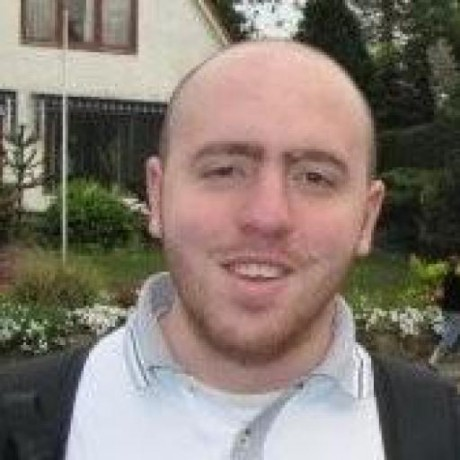
\includegraphics[width=1in,height=1.25in,clip,keepaspectratio]{ismail-el-helw}}]{Ismail El-Helw}
took his MSc at Vrije Universiteit Amsterdam, where he also
did his Ph.D research. Currently, he works with Google in Munich.
\end{IEEEbiography}

\begin{IEEEbiography}[{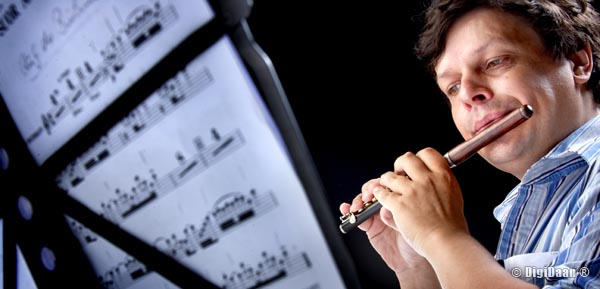
\includegraphics[width=1in,height=1.25in,clip,keepaspectratio]{rutger-hofman-piccolo}}]{Rutger Hofman}
has a Ph.D in Computer Systems from the Universiteit van
Amsterdam. Currently, he is a research programmer at the Vrije Universiteit
Amsterdam.
\end{IEEEbiography}

\begin{IEEEbiography}[{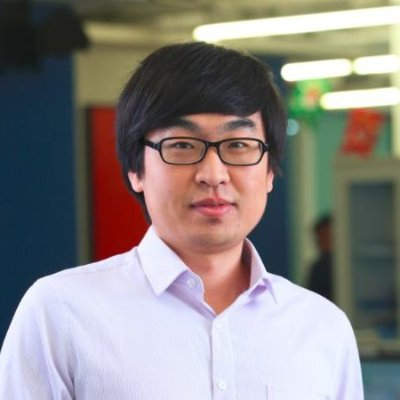
\includegraphics[width=1in,height=1.25in,clip,keepaspectratio]{wenzhe-li}}]{Wenzhe Li}
is a Ph.D student at USC. His research interests include NLP, deep
learning, generative models and its application to graph-structured data.
\end{IEEEbiography}

\begin{IEEEbiography}[{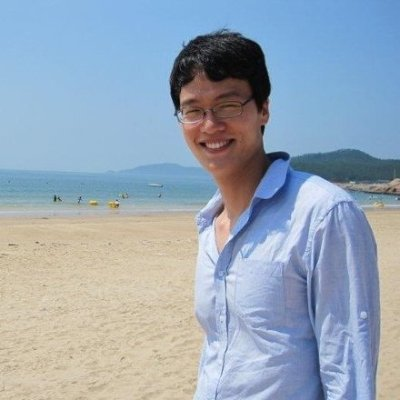
\includegraphics[width=1in,height=1.25in,clip,keepaspectratio]{sungjin-ahn-2}}]{Sungjin Ahn}
is a postdoctoral researcher working with Prof. Yoshua Bengio on
Deep Learning at the University of Montreal. He did his Ph.D. with Professor
Max Welling.
\end{IEEEbiography}

\begin{IEEEbiography}[{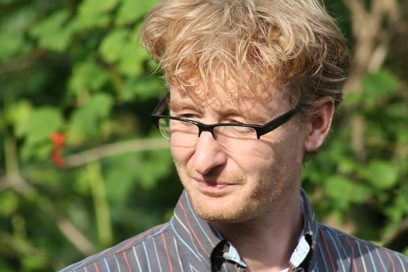
\includegraphics[width=1in,height=1.25in,clip,keepaspectratio]{max-welling}}]{Max Welling}
is a full professor of Machine Learning at the Universiteit van
Amsterdam. He also holds positions at University of California, Irvine, and
the Canadian Institute for Advanced Research.
\end{IEEEbiography}

\begin{IEEEbiography}[{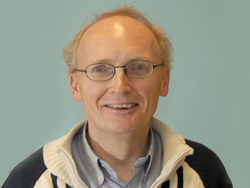
\includegraphics[width=1in,height=1.25in,clip,keepaspectratio]{file-henri-bal}}]{Henri Bal}
is a full professor of Computer Science at Vrije Universiteit,
Amsterdam.
\end{IEEEbiography}

% You can push biographies down or up by placing
% a \vfill before or after them. The appropriate
% use of \vfill depends on what kind of text is
% on the last page and whether or not the columns
% are being equalized.

%\vfill

% Can be used to pull up biographies so that the bottom of the last one
% is flush with the other column.
%\enlargethispage{-5in}



% that's all folks
\end{document}


